% file: AGAT_dump.tex
% Algebraic Geometry, Algebraic Topology, in unconventional ``grande'' format; fitting a widescreen format
% 
% github        : ernestyalumni
% linkedin      : ernestyalumni 
% wordpress.com : ernestyalumni
%
% This code is open-source, governed by the Creative Common license.  Use of this code is governed by the Caltech Honor Code: ``No member of the Caltech community shall take unfair advantage of any other member of the Caltech community.'' 
% 

\documentclass[10pt]{amsart}
\pdfoutput=1
%\usepackage{mathtools,amssymb,lipsum,caption}
\usepackage{mathtools,amssymb,caption}

\usepackage{graphicx}
\usepackage{hyperref}
\usepackage[utf8]{inputenc}
\usepackage{listings}
\usepackage[table]{xcolor}
\usepackage{pdfpages}
%\usepackage[version=3]{mhchem}
%\usepackage{mhchem}

\usepackage{tikz}
\usetikzlibrary{matrix,arrows}

\usepackage{multicol}

% ----------------------------------------------------------------------------------------
% 20180203

\usetikzlibrary{calc}

% ----------------------------------------------------------------------------------------


\hypersetup{colorlinks=true,citecolor=[rgb]{0,0.4,0}}

\oddsidemargin=15pt
\evensidemargin=5pt
\hoffset-45pt
\voffset-55pt
\topmargin=-4pt
\headsep=5pt
\textwidth=1120pt
\textheight=595pt
\paperwidth=1200pt
\paperheight=700pt
\footskip=40pt








\newtheorem{theorem}{Theorem}
\newtheorem{corollary}{Corollary}
%\newtheorem*{main}{Main Theorem}
\newtheorem{lemma}{Lemma}
\newtheorem{proposition}{Proposition}

\newtheorem{definition}{Definition}
\newtheorem{remark}{Remark}

\newenvironment{claim}[1]{\par\noindent\underline{Claim:}\space#1}{}
\newenvironment{claimproof}[1]{\par\noindent\underline{Proof:}\space#1}{\hfill $\blacksquare$}

%This defines a new command \questionhead which takes one argument and
%prints out Question #. with some space.
\newcommand{\questionhead}[1]
  {\bigskip\bigskip
   \noindent{\small\bf Question #1.}
   \bigskip}

\newcommand{\problemhead}[1]
  {
   \noindent{\small\bf Problem #1.}
   }

\newcommand{\exercisehead}[1]
  { \smallskip
   \noindent{\small\bf Exercise #1.}
  }

\newcommand{\solutionhead}[1]
  {
   \noindent{\small\bf Solution #1.}
   }


\title{The Algebraic Geometry Algebraic Topology Dump}
\author{Ernest Yeung \href{mailto:ernestyalumni@gmail.com}{ernestyalumni@gmail.com}}
\date{5 mars 2017}
\keywords{Algebraic Geometry, Algebraic Topology}
\begin{document}

\definecolor{darkgreen}{rgb}{0,0.4,0}
\lstset{language=Python,
 frame=bottomline,
 basicstyle=\scriptsize,
 identifierstyle=\color{blue},
 keywordstyle=\bfseries,
 commentstyle=\color{darkgreen},
 stringstyle=\color{red},
 }
%\lstlistoflistings

\maketitle

From the beginning of 2016, I decided to cease all explicit crowdfunding for any of my materials on physics, math.  I failed to raise \emph{any} funds from previous crowdfunding efforts.  I decided that if I was going to live in \emph{abundance}, I must lose a scarcity attitude.  I am committed to keeping all of my material \textbf{open-sourced}.  I give all my stuff \emph{for free}.   

In the beginning of 2017, I received a very generous donation from a reader from Norway who found these notes useful, through \emph{PayPal}.  If you find these notes useful, feel free to donate directly and easily through \href{https://www.paypal.com/cgi-bin/webscr?cmd=_donations&business=ernestsaveschristmas%2bpaypal%40gmail%2ecom&lc=US&item_name=ernestyalumni&currency_code=USD&bn=PP%2dDonationsBF%3abtn_donateCC_LG%2egif%3aNonHosted}{PayPal}, which won't go through a 3rd. party such as indiegogo, kickstarter, patreon.  Otherwise, under the \emph{open-source MIT license}, feel free to copy, edit, paste, make your own versions, share, use as you wish.    

\noindent gmail        : ernestyalumni \\
linkedin     : ernestyalumni \\
twitter      : ernestyalumni \\

\begin{multicols*}{2}

  
\setcounter{tocdepth}{1}
\tableofcontents



\begin{abstract}
Everything about Algebraic Geometry, Algebraic Topology

\end{abstract}


\part{Algebra; Groups, Rings, R-Modules, Categories}

We should know some algebra.  I will follow mostly Rotman (2010) \cite{JRotman2010}.  

\section{Prime numbers, GCD (greatest common denominator), integers, Euler's totient, Chinese Remainder Theorem, integer divison, modulus, remainders; Euclid's Lemma}

\subsection{Greatest Common Denominator (GCD); Euclid's Lemma}

\begin{theorem}[1.7 of Rotman (2010) \cite{JRotman2010}]\label{Thm:lincombgcd}
	If $a,b\in \mathbb{Z}$, then $\text{gcd}(a,b) \equiv (a,b)=d$ is linear combination of a and b, i.e. $\exists \, s,t \in \mathbb{Z}$ s.t.
	\[
	d= sa + tb
	\]
\end{theorem}
cf. pp.4, Thm. 1.7, Ch. 1 Things Past of Rotman (2010) \cite{JRotman2010}
\begin{proof}
	Let $I:=$ 
	\[
	I :=\lbrace sa+tb|s,t\in \mathbb{Z} \rbrace
	\]
	If $I\neq \lbrace 0 \rbrace$, let $d$ be smallest positive integer in $I$.   \\
	$d\in I$, so $d=sa + tb$ for some $s,t\in \mathbb{Z}$.  
	
	Claim: $I=(d) \equiv \lbrace kd| k\in \mathbb{Z} \rbrace = $ set of all multiples of $d$.  
	
	Clearly $(d)\subseteq I$, since $kd=k(sa+tb) = (ks)a+(kt)b\in I$.  
	
	Let $c\in I$.  
	
	By division algorithm, $c=qd + r$, $0\leq r <d$
	\[
	r=c-qd = s'a+t'b - qsa - qtb = (s'-sq)a + (t'-qt)b \in I
	\]
	If $r\in I$, but $r<d$, contradiction that $\min_{ \substack{ i \in I \\ i>0 \\ } } i =d$.  
	
	So $r=0$, and $d|c=c/d$.  
	\[
	c \in (d), \text{ so } I\subseteq (d) \Longrightarrow I =(d)
	\]
\end{proof}


\begin{theorem}[\textbf{Euclid's Lemma}; 1.10 of Rotman (2010) \cite{JRotman2010}]
	If $p$ prime and $p|ab$, then $p|a$ or $p|b$.  
	
	More generally,  \\
	if prime $p$ divides product $a_1a_2\dots a_n$, \\
	then it must divide at least 1 of the factors $a_i$.  
	
	i.e. (notation),  
	
	If prime $p$, and $ab/p \in \mathbb{Z}$, \\
	then $a/p\in \mathbb{Z}$ or $b/p \in \mathbb{Z}$.  
	
	More generally, \\
	if prime $p$, s.t. $a_1a_2 \dots a_n/p \in \mathbb{Z}$, \\
	then $\exists \, $ 1 \, $a_i$ s.t. $a_i/p \in \mathbb{Z}$
\end{theorem}
\begin{proof}
	If $p\nmid a$, i.e. $a/p \notin \mathbb{Z}$, then $\text{gcd}(p,a)  \equiv (p,a) =1$.  
	
	From Thm. \ref{Thm:lincombgcd}, 
	\[
	1 = sp+ta
	\]
	\[
	\Longrightarrow b = spb + tab = p(sb+td)
	\]
	$ab/p$ and so $ab=pd$, so $b=spb+tdp$, i.e. $b$ is a multiple of $p$ ($b/p \in \mathbb{Z} \equiv p | b$).  
	
	
	
	
\end{proof}

\begin{corollary}[1.11 of Rotman (2010) \cite{JRotman2010}]\label{Cor:relprimefactors}
	Let $a,b,c \in \mathbb{Z}$.  
	
	If $c,a$ relatively prime, i.e. $\text{gcd}(c,a)=1$, and if $c|ab \equiv ab/c\in \mathbb{Z}$,
	then $c|b \equiv b/c \in \mathbb{Z}$
\end{corollary}
\begin{proof}
	\[
	\text{gcd}(c,a)=1 = sc+ta \Longrightarrow b=sbc + tab = sbc + t(qc) = c(sb+tq) \Longrightarrow b/c = sb+tq 
	\]
\end{proof}



\begin{theorem}[1.26 of Rotman (2010) \cite{JRotman2010}]
	If $\text{gcd}(a,m) \equiv (a,m) = 1$, then $\forall \, b \in \mathbb{Z}$, $\exists \, x $ s.t. 
	\[
	ax = b\mod{m}
	\]
	In fact, $x=sb$, where $sa\equiv 1\mod{m}$
\end{theorem}
\begin{proof}
	$\gcd(a,m) = 1=sa+tm$.   
	
	Then $b=b\cdot 1=  b(sa+tm) = sab+tmb$ or $b=tbm+sab$ or $a(sb) = -tbm + b$.  
	
	So $a(sb)\mod{m}=b$.  
	
	Let $x:= sb$ and so $ax \mod{m}=b$.   \\
	Now suppose $x \neq sb$ s.t. $ax\mod{m}=b$.  Then $ax=qm +b$.  From $a(sb) \mod{m}=b$, we also get $a(sb) = q'm + b$.  Then $a(x-sb) \mod{m}=0$, so $m|a(x-sb) \equiv a(x-sb)/m\in \mathbb{Z}$.  
	
	By Corollary \ref{Cor:relprimefactors} (which says, if $\gcd(c,a)=1$ and if $ab/c\in\mathbb{Z}$, then $b/c \in \mathbb{Z}$), 
	since $\gcd(m,a) = (m,a)=1$, and since $a(x-sb)/m \in \mathbb{Z}$, then $(x-sb)/m\in\mathbb{Z}$.  So $(x-sb)=qm$ or $(sb)\mod{m} = x$.  
	
	
\end{proof}



\begin{proposition}[3.1 of Scheinerman (2006) \cite{Sche2006}]\label{Prop:commongcd}
	Let $a,b\in \mathbb{Z}$, let $c=a\mod{b}$, i.e. $a=qb+c$ s.t. $0\leq c <b$.  
	
	Then 
	\begin{equation}
	\text{gcd}(a,b) = \text{gcd}(b,c)
	\end{equation}
\end{proposition}
cf. Sec. 3.3 Euclid's method of Scheinerman (2006) \cite{Sche2006}

\begin{proof}
	If $d$ common divisor of $a,b$, i.e. $a/d, b/d \in \mathbb{Z} \equiv d|a, d|b$.   \\
	$c/d \in \mathbb{Z} \equiv d|c$ since $c=a-qb$.  
	
	If $d$ is common divisor of $b,c$, i.e. $d|b, d|c \equiv c/d, b/d\in\mathbb{Z}$, \\
	then $d|a \equiv a/d \in \mathbb{Z}$ since $a=qb+c$.  So set of common divisors of $a,b$ same as set of common divisors of $b$ and $c$.  
	
	Then $\text{gcd}(a,b) = \text{gcd}(b,c)$.  
\end{proof}




\subsection{Euler's totient; relatively prime}

\begin{definition}
	if $a,b \in \mathbb{Z}$, \\
	a \textbf{divisor} of b, if $\exists \, d\in \mathbb{Z}$ s.t. $b=ad$.   \\
	Also, $a$ \textbf{divides} $b$ or $b$ multiple of $a \equiv a | b$.  \\
	$a|b \equiv b/a \in \mathbb{Z}$  
\end{definition}
cf. pp. 3 of Ch. 1 Things Past, Sec. 1.1 Some Number Theory of Rotman (2010) \cite{JRotman2010}.  

cf. Ch. 5 Arrays, Sec. 5.1 Euler's totient of Scheinerman (2006) \cite{Sche2006}

For 
\[
\begin{aligned}
& \varphi : \mathbb{Z}^+ \to \mathbb{Z}^+ \\ 
& \varphi : n \mapsto \varphi(n) := \text{ number of elements of $\lbrace 1,2, \dots n \rbrace$ that are relative prime to $n$ } = | \lbrace i | i \in \lbrace 1,2, \dots n \rbrace , (n,i)=1 \text{ or equivalently } n \propto i \rbrace |
\end{aligned}
\]

e.g. $\varphi(10) = 4$ since $\varphi(10) = | \lbrace 1,3,7,9\rbrace|$.  

we want $|(a,b) | 1 \leq a,b, \leq n , \text{gcd}(a,b) \equiv (a,b) = 1 |$.  

\[
p_n = \frac{1}{n^2} \left[ -1 + 2\sum_{i=1}^n \varphi(k) \right] = \text{ probability that 2 integers, chosen uniformly and independently from $\lbrace 1,2,\dots n\rbrace$ are relatively prime }
\]

If $p$ is prime, $\forall \, i \in \lbrace 1,2,\dots p \rbrace$, $(p,i) \equiv \text{gcd}(p,i)=1$, i.e. relatively prime to $p$, except 1 $i\in \lbrace 1,2,\dots p\rbrace$.  

Therefore 
\[
\varphi(p) = p-1
\]
Consider $\varphi(p^2)$.  

$\lbrace 1,2,\dots p^2\rbrace$, only numbers \emph{not} relatively prime to $p^2$ are multiples of $p$ since \\
$p,2p, 3p, \dots p^2$ all divide $p^2$, i.e. $p|p^2, 2p|p^2 \dots (p-1)p | p^2 \equiv p^2 /p , p^2 /2p , \dots p^2 / p(1-p)$.  

Assume $\varphi(p^n) = p^2 - p^{n-1} = p^{n-1}(p-1)$.  

\[
\varphi(p^{n+1}) = \varphi(pp^{n}) = p^n\varphi(p) = p^n(p-1)
\]
Therefore,
\begin{proposition}[5.1]
	Let $p$ prime, $n\in \mathbb{Z}^+$
\end{proposition}


e.g. $\varphi(77)$.  

$\forall \, n $ s.t. $1\leq n \leq 77$.  
\[
\begin{aligned}
& \text{gcd}(n,77)=1 \\ 
& \text{gcd}(n,7)=1 \\ 
& \text{gcd}(n,11)=1  
\end{aligned}
\]
By Prop. \ref{Prop:commongcd}, 
\[
\begin{aligned}
& \text{gcd}(n,7) = \text{gcd}(7, n\mod{7}) \\ 
& \text{gcd}(n,11) = \text{gcd}(11, n\mod{11}) 
\end{aligned}
\]


Scheinerman (2006) \cite{Sche2006}



\subsubsection{Chinese Remainder Theorem}

\begin{theorem}
	If $m,m'$ relatively prime (i.e. $\gcd(m,m')=1$), then for 
	\[
	\begin{aligned}
	& x \equiv b \mod{m} \\ 
	& x\equiv b'\mod{m'}
	\end{aligned}
	\]
	i.e. given $b,b'm,m'$, and wanting to find $x$, 
	$\exists \, x$ and $\forall \, 2 x$'s, $x=x'\mod{mm'}$.  
\end{theorem}

\begin{proof}
	$x = b'ms + bm's'$
\end{proof}

cf. Ch. 1 Things Past, Thm. 1.28 of Rotman (2010) \cite{JRotman2010}, pp. 68 Thm. 5.2 (Chinese Remainder) of Scheinerman (2006) \cite{Sche2006}.  




\section{Groups; normal subgroups}  

\begin{definition}[normal subgroup $K \lhd G$] \qquad \, \\
	\textbf{normal subgroup} $K$ of $G \equiv K \lhd G$   - 
	
	subgroup $K\subset G$, if $\forall \, k \in K$, $\forall \, g \in G$, 
	\[
	gkg^{-1} \in K
	\]
\end{definition}

\begin{definition}[quotient group] \qquad \, \\
	\textbf{quotient group} $G\mod{K} \equiv G/K$ -  
	
	if $G/K = $ family of all left cosets of subgroups $K\subset G = $
	\[ 
	= \lbrace gK | g\in G, K = \lbrace gk | k \in K \rbrace 
	\]
	and 
	
	$K = $ normal subgroup of $G$, i.e. $K \lhd G$, and so 
	\[
	aK bK = abK \qquad \, \forall \, a,b \in G, 
	\]
	so $G/K $ group.  
\end{definition}






% 20170925 

\begin{definition}[exact sequence of groups]
	\textbf{exact sequence} if $\text{im}f_{n+1} = \text{ker}f_n$  \qquad \, $\forall \, n $ for sequence of group homomorphisms and groups 
\begin{equation}
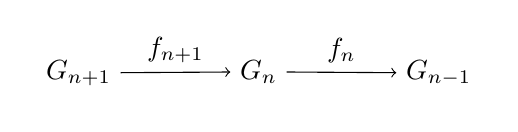
\begin{tikzpicture}
%\matrix(m)[matrix of math nodes, row sep=3em, column sep=3em, text height=1.5ex, text depth=0.25ex]
\matrix(m)[matrix of math nodes, row sep=4em, column sep=4em]
{
	G_{n+1}   &  G_n & G_{n-1} \\
};
%\path[->,font=\scriptsize]
\path[->]
(m-1-1) edge node[auto]{$f_{n+1}$} (m-1-2)
(m-1-2) edge node[auto]{$f_n$} (m-1-3);
\end{tikzpicture} 
\end{equation}
\end{definition}

	
\begin{theorem}
	\begin{enumerate}
		\item \[
		\begin{tikzpicture}
		%\matrix(m)[matrix of math nodes, row sep=3em, column sep=3em, text height=1.5ex, text depth=0.25ex]
		\matrix(m)[matrix of math nodes, row sep=4em, column sep=4em]
		{
			1   &  A & B \\
			%\path[->,font=\scriptsize]
		};
		\path[->]
		(m-1-2) edge node[auto]{$f$} (m-1-3);
		\end{tikzpicture} 
		\]
		\item \[
		\begin{tikzpicture}
		%\matrix(m)[matrix of math nodes, row sep=3em, column sep=3em, text height=1.5ex, text depth=0.25ex]
		\matrix(m)[matrix of math nodes, row sep=4em, column sep=4em]
		{
			B   &  C & 1 \\
		};
		%\path[->,font=\scriptsize]
		\path[->]
		(m-1-1) edge node[auto]{$g$} (m-1-2);
		\end{tikzpicture} 
		\]
		\item \[
		\begin{tikzpicture}
		%\matrix(m)[matrix of math nodes, row sep=3em, column sep=3em, text height=1.5ex, text depth=0.25ex]
		\matrix(m)[matrix of math nodes, row sep=4em, column sep=4em]
		{
			1 & A   &  B & 1 \\
		};
		%\path[->,font=\scriptsize]
		\path[->]
		(m-1-2) edge node[auto]{$h$} (m-1-3);
		\end{tikzpicture} 
		\]
		
	\end{enumerate}
\end{theorem}

\begin{proof}
	\begin{enumerate}
		\item $\text{im}(1\to A)=1$, since $1\to A$ is a group homomorphism $((1\to A)(1) = 1_A)$.  \\
		if $1\to A \xmapsto[]{f} B$ exact, $\text{ker}f = \text{im}(1\to A)=1$, so if $f(x)=1$, $x=1$, $f$ injective.  \\
		If $f$ injective, $\text{ker}f=1$.  $1=\text{im}(1\to A)$.  $1\to A \xmapsto{f}B$, exact.  
		\item $\text{ker}(C\to 1) = C$, by def. of $C\to 1$ \\
		if $B \xmapsto{g} C \to 1$ exact, $\text{im}g = g(B) = \text{ker}(C\to 1)= C$.  $g(B) = C$ implies $g$ surjective.  \\
		If $g$ surjective, $g(B) = C =\text{ker}(C\to 1)$.  $B\xmapsto{g} C \to 1$ exact.  
		\item From (i), $1\to A \xmapsto{h}B$ exact iff $h$ injective.  
		From (ii), $A\xmapsto{h}B \to 1$, exact iff $h$ surjective.  \\
		$h$ isomorphism.  
	\end{enumerate}
\end{proof}








% 20170925 END

\subsection{1st, 2nd, 3rd Isomorphism Theorems}

\begin{theorem}[1st Isomorphism Theorem (Modules) Thm. 7.8 of Rotman (2010) \cite{JRotman2010}]
	If $f:M\to N$ is $R$-map of modules, then $\exists \, R$-isomorphism s.t. 
	\begin{equation}
	\begin{aligned}
	& \varphi : M /\text{ker}f \to \text{im}f \\ 
	& \varphi: m + \text{ker}f \mapsto f(m)
	\end{aligned} \qquad \qquad \, 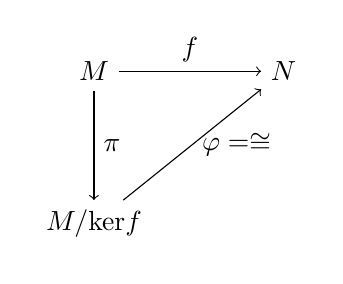
\begin{tikzpicture}
	%\matrix(m)[matrix of math nodes, row sep=3em, column sep=3em, text height=1.5ex, text depth=0.25ex]
	\matrix(m)[matrix of math nodes, row sep=4em, column sep=4em]
	{
		M   &  N \\
		M/\text{ker}f  &  \\};
	%\path[->,font=\scriptsize]
	\path[->]
	(m-1-1) edge node[auto]{$f$} (m-1-2)
	edge node[auto]{$\pi$} (m-2-1) 
	(m-2-1) edge node[right]{$\varphi = \cong$} (m-1-2);
	\end{tikzpicture} 
	\end{equation}
	%Essentially, 
	%\begin{equation}
	
	%\end{equation}
\end{theorem}

\begin{proof}
	View $M,N$ as abelian groups.  
	
	Recall natural map $ \begin{aligned} & \quad \\ 
	& \pi : M \to M/N \\
	& m\mapsto m + N \end{aligned}$  
	
	Define $\varphi$ s.t. $\varphi \pi = f$.  
	
	($\varphi$ well-defined).  Let $m+\text{ker}f = m' + \text{ker}f$, $m,m' \in M$, then $\exists \,  n \in \text{ker}f$ s.t. $m=m'+n$.  
	\[
	\varphi(m+\text{ker}f) = \varphi\pi (m) = f(m) = f(m' +n ) = f(m') + f(n) = \varphi \pi(m') + 0 = \varphi(m' + \text{ker}f )
	\]
	$\Longrightarrow \varphi $ well-defined.  
	
	($\varphi$ surjective).  Clearly, $\text{im}\varphi \subseteq  \text{im} f$.   \\
	Let $y\in \text{im}f$.  So $\exists \,  m \in M$ s.t. $y=f(m)$.  $f(m) = \varphi \pi (m) = \varphi(m+\text{ker}f) = y$.  So $y\in \text{im}\varphi$.  $\text{im}f\subseteq \text{im}\varphi$.  \\
	$\Longrightarrow \varphi $ surjective.  
	
	($\varphi$ injective)  If $\varphi(a+\text{ker}f) = \varphi(b+\text{ker}f)$, then 
	\[
	\begin{gathered}
	\varphi\pi(a) = \varphi\pi(b) \text{ or } f(a) = f(b) \text{ or } 0 = f(a) -f(b) = f(a-b) \text{ so } a-b \in \text{ker}f
	(a-b) + \text{ker}f = \text{ker}f \text{ so } a + \text{ker}f = b +\text{ker}f 
	\end{gathered}
	\]
	$\varphi$ isomorphism.  
	
	$\varphi$ $R$-map.  $\varphi(r(m+N)) = \varphi(rm+N) = f(rm)$.    \\
	Since $f$ $R$-map, $f(rm) = rf(m) = r\varphi(m+N)$.  $\varphi$ is $R$-map indeed.  
	
	
\end{proof}


\begin{theorem}[2nd Isomorphism Theorem (Modules) Thm. 7.9 of Rotman (2011) \cite{JRotman2010}]
	If $S,T$ are submodules of module $M$, i.e. $S,T \in M$, then $\exists \, $ $R-$isomorphism  
	\begin{equation}
	\begin{gathered}
	S/(S\cap T) \to (S+T)/T
	\end{gathered} \qquad \, 
	\qquad \qquad \, 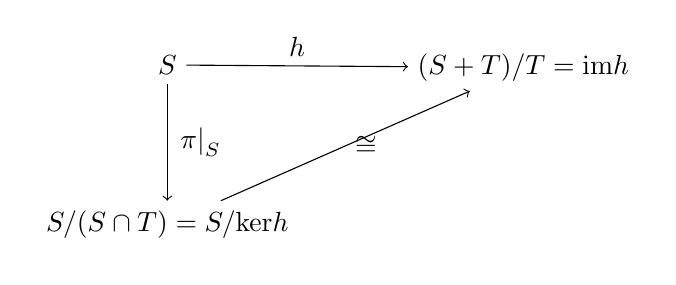
\begin{tikzpicture}
	\matrix(m)[matrix of math nodes, row sep=4em, column sep=4em]
	{
		S   &  (S+T)/T = \text{im}h \\
		S/(S\cap T) = S/\text{ker}h  &  \\};
	\path[->]
	(m-1-1) edge node[auto]{$h$} (m-1-2)
	edge node[auto]{$\left. \pi \right|_S$} (m-2-1) 
	(m-2-1) edge node[right]{$ \cong$} (m-1-2);
	\end{tikzpicture} 
	\end{equation}
\end{theorem}

\begin{proof}
	Let natural map $\pi : M \to M/T$.   \\
	\phantom{Let} So $\text{ker}\pi = T$.  
	
	Define $h:= \left. \pi \right|_S$, so $h: S\to M/T$, so $\text{ker}h = S\cap T$, 
	\[
	(S+T)/T = \lbrace (s+t) + T | a\in S+T, s\in S, t\in T \rbrace
	\]
	i.e. $(S+T)/T$ consists of all those cosets in $M/T$ having a representation in $S$.  
	
	By 1st. isomorphism theorem, 
	\[
	S/S\cap T \xrightarrow{ \cong} (S+T)/T
	\]
	
\end{proof}  % END of pf. of 2nd Isomorphism Theorem (Modules) Thm. 7.9 of Rotman (2011)

\begin{theorem}[3rd Isomorphism Theorem (Modules) Thm. 7.10 of Rotman (2011) \cite{JRotman2010}]
	If $T\subseteq S \subseteq M$ is a tower of submodules, then $\exists \, $ $R$-isomorphism
	\begin{equation}
	\begin{gathered}
	(M/T)/(S/T) \to M/S
	\end{gathered} \qquad \,  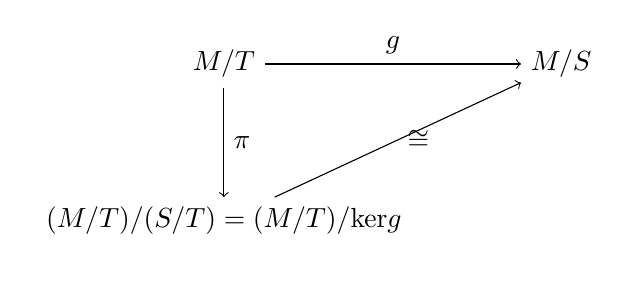
\begin{tikzpicture}
	\matrix(m)[matrix of math nodes, row sep=4em, column sep=4em]
	{
		M/T   &  M/S\\
		(M/T)/(S/ T) = (M/T)/\text{ker}g  &  \\};
	\path[->]
	(m-1-1) edge node[auto]{$g$} (m-1-2)
	edge node[auto]{$ \pi $} (m-2-1) 
	(m-2-1) edge node[right]{$ \cong$} (m-1-2);
	\end{tikzpicture} 
	\end{equation}
\end{theorem}

\begin{proof}
	Define $g:M/T \to M/S$ to be \textbf{coset enlargement}, i.e. 
	\begin{equation}
	g:M +T \mapsto m+S
	\end{equation}
	$g$ well-defined: if $m+T = m'+T$, then $m-m' \in T\subseteq S$, and $m+S = m'+S \Longrightarrow g(m+T) = g(m'+T)$
	
	$\text{ker}g = S/T$ since 
	\[
	\begin{aligned}
	& g(s+T) = s+S = S  \qquad \, (S/T \subseteq \text{ker}g)   \\
	& g(m+T) = m + S = 0 = S = s + S, \text{ so } m=s \Longrightarrow \text{ker}g \subseteq S/T
	\end{aligned}
	\]
	$\text{im}g = M/S $ since 
	\[
	\begin{aligned}
	& g(m+T) = m+S \Longrightarrow \text{ im}g \subseteq M/S \\ 
	& m+S = g(m+T)
	\end{aligned}
	\]
	Then by 1st isomorphism, and commutative diagram, done.  
\end{proof} % END of pf. of 3rd Isomorphism Theorem (Modules) Thm. 7.10 of Rotman (2011) 



\section{R-modules}

\begin{definition}[R-homomorphism (or R-map)]
	If ring $R$, $R$-modules $M,N$, then \\
	function $f: M\to N$, \\
	if $\forall \, m, m' \in M$, $\forall \, r\in R$, 
	\[
	\begin{gathered}
	f(m+m') = f(m) + f(m') \\ 
	f(rm) = rf(m)
	\end{gathered}
	\]
\end{definition}

\begin{definition}[quotient module $M/N$] \qquad \, \\ 
	\textbf{quotient module} $M/N$  -
	
	For submodule $N$ of $R$-module $M$, then, \\
	remember $M$ abelian group, $N$ subgroup, \\
	quotient group $M/N$ equipped with scalar multiplication 
	\[
	\begin{gathered}
	r(m+N) = rm+N \\ 
	M/N = \lbrace m +N | m \in M \rbrace
	\end{gathered}
	\]
	\textbf{natural map} 
	\begin{equation}
	\begin{aligned}
	& \pi : M \to M /N \\ 
	& m\mapsto m + N 
	\end{aligned}
	\end{equation}
	easily seen to be $R$-map.  
	
	Scalar multiplication in quotient module well-defined: \\
	If $m+N=m'+N$, $m-m' \in N$, so $r(m-m') \in N$ (because $N$ submodule), so 
	\[
	rm - rm' \in N \text{ and } rm+ N = rm' +N
	\]
	
	
\end{definition}


\begin{proposition}[7.15 of Rotman (2010) \cite{JRotman2010}]  
	\begin{enumerate}
		\item[(i)] $S \bigsqcup T \simeq M$ 
		\item[(ii)] $\exists \, $ injective $R$-maps $\begin{aligned} & \quad \\ 
		& i : S\to M \\ 
		& j :T \to M \end{aligned}$, s.t. 
		
		\begin{equation}
		\begin{gathered} 
		M = \text{im}(i) + \text{im}(j)  \text{ and } \\ 
		\text{im}(i) \bigcap \text{im}(j) = \lbrace 0 \rbrace  
		\end{gathered}
		\end{equation}
		\item[(iii)] $\exists \, $ R-maps 
		\[
		\begin{aligned}
		& i : S\to M \\ 
		& j : T\to M 
		\end{aligned}
		\]
		s.t. $\forall \, m \in M$, $\exists \, !$ 
		\[
		\begin{aligned}
		& s \in S \\ 
		& t \in T 
		\end{aligned}
		\] with $m=is + jt$.  
		\item[(iv)] $\exists \, $ R-maps 
		\[
		\begin{gathered}
		\begin{aligned}  & i: S\to M \\ 
		& j:T \to M \end{aligned} \qquad \, \begin{aligned}
		& p : M \to S \\ 
		& q : M \to T \end{aligned}
		\end{gathered}
		\]
		s.t. 
		\[
		\begin{gathered}
		\begin{aligned}
		& pi = 1_S \\ 
		& qj = 1_T 
		\end{aligned} \qquad \ , \begin{aligned}
		& pj = 0  \\
		& qi = 0 
		\end{aligned} \qquad \, ip + jq = 1_M
		\end{gathered}
		\]
	\end{enumerate}
\end{proposition}

\begin{proof}
	\begin{itemize}
		\item (i)$\to$ (ii)  Given $S \bigsqcup T \simeq  M$,  \\ 
		let $\varphi : S \bigsqcup T \to   M$ be this isomorphism.  
		
		Define
		\[
		\begin{aligned}
		& i:= \varphi \lambda_S \qquad \, & (\lambda_S : s\mapsto (s,0)) \qquad \, & i :S \to M \\ 
		& j:= \varphi \lambda_T \qquad \, & (\lambda_T : t\mapsto (0,t)) \qquad \, & j :T \to M 
		\end{aligned}
		\]
		$i,j$ are injections, being composites of injections.  
		
		If $m\in M$, $\exists \, ! \, (s,t) \in S\bigsqcup T$, s.t. $\varphi(s,t)=m$.  
		
		Then 
		\[
		m = \varphi(s,t) = \varphi((s,0) + (0,t)) = \varphi\lambda_S(s)  \varphi \lambda_T(t) = is + jt \in \text{im}(i) + \text{im}(j)
		\]
		
		Let $c\in \text{im}(i) + \text{im}(j)$.  Since $\begin{aligned}  & \quad \\ 
		& i : S\to M \\
		& j : T \to M \end{aligned}$, $c\in M$.  
		
		$\Longrightarrow M = \text{im}(i) + \text{im}(j)$.  
		
		
		
		If $x\in \text{im}(i) \bigcap \text{im}(j)$, 
		\[
		\begin{aligned}
		& x = i(s) \text{ for some } s\in S \\ 
		& x = j(t) \text{ for some } t\in T  
		\end{aligned}
		\]
		
		\[
		\begin{gathered}
		is=jt = \varphi \lambda_S(s) = \varphi \lambda_T(t) = \varphi(s,0) = \varphi(0,t) 
		\end{gathered}
		\]
		$\varphi$ isomorphism, so $\exists \, \varphi^{-1}$ $\Longrightarrow (s,0) = (0,t)$, so $s=t=0$.  $x=0$  
		\item (ii)$\to $ (iii) Given $\begin{aligned} & \quad \\ & i:S\to M \\ & j:T\to M \end{aligned}$, s.t. $M= \text{im}(i) + \text{im}(j)$, so \\
		
		$\forall \, m \in M$, $m=i(s) + j(t)$ for some $s\in S,t\in T$.  
		
		Suppose $\begin{aligned} & \quad \\ 
		& s' \in S \\
		& t' \in T \end{aligned}$, s.t. $m=i(s'_ + j(t')$.  
		\[
		i(s-s') = j(t-t') \in \text{im}(i) \bigcap \text{im}(j) = \lbrace 0 \rbrace
		\]
		So $s=s',t=t'$, since $i,j$ injective.  
		\item (iii)$\to$ (iv)   
		
		Given $\forall \, m \in M$, $\exists \, ! \, s\in S,t\in T$ s.t. 
		\[
		m=i(s) + j(t)
		\]
		Define 
		\[
		\begin{aligned}
		& p:M \to S \\ 
		& p(m) := s
		\end{aligned} \qquad \, \begin{aligned}
		& q: M \to T \\ 
		& q(m) := t
		\end{aligned}
		\]
		\[
		\begin{aligned}
		& pi(s) = s \\ 
		& qj(t) = t 
		\end{aligned} \qquad \, \begin{aligned}
		& pj(t) =0  \\
		& qi(s) = 0 \end{aligned} \qquad \, 
		(ip+jq)(m) = ip(m) + jq(m) = i(s) + j(t) = m 
		\]
	\end{itemize}
\end{proof}

\section{Categories; Category Theory}  

\subsection{Categories}

cf. 7.2 Categories of Rotman (2010) \cite{JRotman2010}

\subsubsection{Russell paradox, Russell set}  

\begin{definition}[Russell set]
	Russell set  - set $S$ that's not a member of itself, i.e. $S\notin R$
\end{definition}

If $R$ is family of all Russell sets,  \\
Let $X\in R$.  Then $X\notin X$.  But $X\in R$.  $X\notin R$.  \\
Let $R\notin R$.  Then $R$ in family of Russell Sets.  $R\in R$.  Contradiction.  

Then consider \emph{class} as primitive term, instead of set.  

\begin{definition}[Category]
	Category $\mathcal{C}$ (Rotman's notation) $\equiv \mathbf{C}$ (my notation), consists of class $\text{obj}(\mathcal{C})$ (Rotman's notation) $\equiv \text{Obj}(\mathbf{C}) \equiv \text{Obj}\mathbf{C}$ (my notation) of objects, set of  \textbf{morphisms} $\text{Hom}(A,B)$ $\forall \,  (A,B)$ of ordered tuples of objects, composition 
	\[
	\begin{gathered} 
	\text{Hom}(A,B)\times \text{Hom}(B ,C) \to \text{Hom}(A,C) \\
	(f,g)\mapsto gf \end{gathered}
	\], s.t.
	\begin{enumerate}
		\item $\exists \, \mathbf{1}$, $\forall \, f:A\to B$, $\exists \, \begin{aligned} & \quad \\ 
		1_A : A \to A \\
		1_B : B \to B \end{aligned}$, s.t. $1_B \cdot f = f= f\cdot 1_A$, and 
		\item associativity, $\forall \, \begin{aligned} & \quad \\
		& f : A\to B \\
		& g: B\to C \\
		& h: C\to D \end{aligned}$, then $h\circ (g\circ f) = (h\circ g) \circ f$ 
	\end{enumerate}
	
	In summary, 
	\begin{equation}
	\mathbf{C} := (\text{Obj}(\mathbf{C}), \text{Mor}\mathbf{C}, \circ, \mathbf{1}) \equiv (\text{Obj}\mathbf{C}, \text{Mor}\mathbf{C}, \circ_{\mathbf{C}}, \mathbf{1}_{\mathbf{C}})
	\end{equation}
	s.t. 
	\[
	\text{Mor}\mathbf{C} = \bigcup_{A,B \in \text{Obj}\mathbf{C}} \text{Hom}(A,B)
	\]
\end{definition}

Examples (7.25 of Rotman (2010)\cite{JRotman2010}): 
\begin{enumerate}
	\item[(i)] $\mathbf{C} = \mathbf{\text{Sets}}$  
	\item[(ii)] $\mathbf{C} = \mathbf{\text{Groups}} = \mathbf{\text{Grps}}$ 
	\item[(iii)]  $\mathbf{C} = \mathbf{\text{CommRings}}$
	\item[(iv)]  $\mathbf{C} = {}_R\textbf{Mod}$, if $R=\mathbb{Z}$, ${}_{\mathbb{Z}}\textbf{Mod} = \textbf{Ab}$, i.e. $\mathbb{Z}-$modules are just abelian groups.   
	\item[(v)] $\mathbf{C} =\textbf{PO}(X)$, If partially ordered set $X$, regard $X$ as category, s.t. $\textbf{Obj}, \textbf{PO}(X) = \lbrace x | x\in X\rbrace$, $\forall \, \text{Hom}(x,y) \in \textbf{Mor}_{\textbf{PO}}(X)$, $\text{Hom}(x,y) = \begin{cases} \emptyset & \text{ if } x \npreceq y \\  \kappa_y^x & \text{ if } x \preceq y   \end{cases}$ where $\kappa_y^x \equiv $ unique element in $\text{Hom}$ set when $x \preceq y$) s.t. 
	\[
	\kappa_z^y \kappa_y^x  =\kappa_z^x
	\]
	Also, notice that 
	\[
	1_x = \kappa_x^x
	\]
\end{enumerate}

\begin{definition}[isormorphisms or equivalences]
	$f:A\to B$, $f\in \text{Hom}(A,B)$, if $\exists \, $ \textbf{inverse} $g:B\to A$, $g\in \text{Hom}(B,A)$, s.t. 
	\[
	\begin{aligned}
	& gf = 1_A \\ 
	& fg = 1_B
	\end{aligned}
	\]
	and if $\mathbf{C} = \textbf{Top}$, equivalences (isomorphisms) are homeomorphisms.  
\end{definition}

Feature of category ${}_R\textbf{Mod}$ not shared by more general categories: \emph{Homomorphisms can be added.}

\begin{definition}[pre-additive Category]
	category $\mathbf{C}$
\end{definition} 





%--------------------------------------------------------------------------------
% 20180202 
%-------------------------------------------------------------------------------

We can force 2 overlapping subsets $A,B$ to be disjoint by ``disjointifying'' them: e.g. consider $(A\cup B) \times \lbrace 1,2 \rbrace$, consider $\begin{aligned} & \quad \\
& A' = A\times \lbrace 1 \rbrace \\
& B' = B\times \lbrace 2 \rbrace \end{aligned}$.

\[
\Longrightarrow A' \cap B' = \emptyset 
\]
since $(a,1) \neq (b,2)$ \, $\forall \, a \in A$, $\forall \, b \in B$.

Let bijections $\begin{aligned} & \quad \\
& \alpha : A \to A' \\
& \beta : B \to B' \end{aligned}$, \qquad \, $\begin{aligned} & \quad \\
& \alpha : a \mapsto (a,1) \\
& \beta : b\mapsto (b,2) \end{aligned}$, denote $A'\bigcup B' \equiv A \coprod B$.

From Rotman (2010) \cite{JRotman2010}, pp. 447,
\begin{definition}
	\textbf{coproduct} $A \coprod B \equiv C \in \text{Obj}(\mathcal{C})$
\end{definition}

In my notation,

\textbf{coproduct}
\begin{equation}
\begin{aligned}
& (\mu_1 , A_1 \coprod A_2 ) \\ 
& (\mu_2 , A_1 \coprod A_2 ) 
\end{aligned}
\end{equation}
where injection (morphisms)
\begin{equation}
\begin{aligned}
& \mu_1 : A_1 \to A_1 \coprod A_2 \\ 
& \mu_2 : A_1 \to A_1 \coprod A_2 
\end{aligned}
\end{equation}
s.t.
\[
\forall \, A \in \text{Obj}\mathbf{A}, \, \forall \, f_1 ,f_2 \in \text{Mor}\mathbf{A} \text{ s.t. } \begin{aligned} & \quad \\
& f_1 : A_1 \to A \\
& f_2 : A_2 \to A \end{aligned}
\]
then
\begin{equation}
\begin{gathered}
\exists \, ! [ f_i ] \equiv [f_1, f_2 ] \in \text{Mor} \mathbf{A}, \, [f_1, f_2] : A_1 \coprod A_2 \to A \text{ s.t. } \\ 
\begin{aligned}
& [f_1,f_2] \mu_1 = f_1 \\ 
& [f_1,f_2] \mu_2 = f_2 \\
\end{aligned}
\end{gathered}
\end{equation}
i.e. 
\begin{equation}
\begin{gathered}
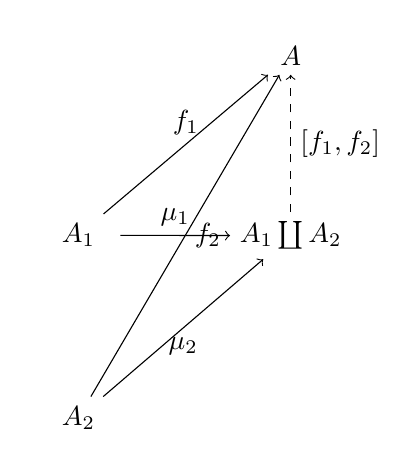
\begin{tikzpicture}
\matrix (m) [matrix of math nodes, row sep=5em, column sep=4em, minimum width=3em]
{
	& A  \\ 
	A_1  &  A_1 \coprod A_2   \\
	A_2 & \\
};
\path[->]
(m-2-1) edge node [above] {$f_1$} (m-1-2)
edge node [above] {$\mu_1$} (m-2-2)
(m-3-1) edge node [right] {$f_2$} (m-1-2)
edge node [below] {$\mu_2$} (m-2-2)
;
\path[dashed,->]
(m-2-2) edge node [right] {$[f_1,f_2]$} (m-1-2)
;
\end{tikzpicture}
\end{gathered}
\end{equation}

So to generalized, for $i\in I$, (finite set $I$?)

\textbf{coproduct} $(\mu_j, \coprod_{i\in I} A_i)_{j\in I}$, where \\
(family of) injection (morphisms) $\mu_j : A_j \to \coprod_{i \in I } A_i$

s.t.

\[
\forall \, A \in \text{Obj}\mathbf{A}, \, \forall \, f_i \in \text{Mor}\mathbf{A}, \, i \in I, \, f_i : A_i \to A
\]
then
\begin{equation}
\begin{gathered}
\exists \, ! \, [f_i ] \equiv [f_i]_{i\in I} \in \text{Mor}\mathbf{A} , \, [f_i] : \coprod_{i\in I} A_i \to A \text{ s.t. } \\ 
[f_i] \mu_j = f_j \qquad \, \forall \, j \in I
\end{gathered}
\end{equation}
i.e.

\begin{equation}
\begin{gathered}
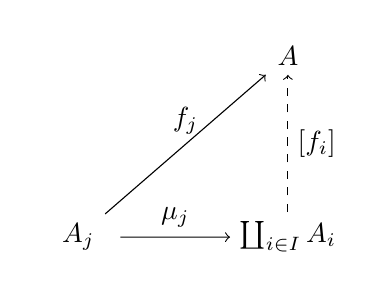
\begin{tikzpicture}
\matrix (m) [matrix of math nodes, row sep=5em, column sep=4em, minimum width=3em]
{
	& A  \\ 
	A_j  & \coprod_{i\in I} A_i   \\
};
\path[->]
(m-2-1) edge node [above] {$f_j$} (m-1-2)
edge node [above] {$\mu_j$} (m-2-2)
;
\path[dashed,->]
(m-2-2) edge node [right] {$[f_i]$} (m-1-2)
;
\end{tikzpicture} 
\end{gathered}
\end{equation}



For notation purposes only, recall that it's denoted the sets $\text{Hom}(A,B)$ in ${}_R\textbf{Mod}$ by
\[
\text{Hom}_R(A,B)
\]
i.e., in my notation, for $A,B \in \text{Obj}{ {}_R \textbf{Mod}}$, $\text{Hom}(A,B) \subset \text{Mor}( {}_R\textbf{Mod})$, $\text{Hom}(A,B) \equiv \text{Hom}_R(A,B)$

\begin{definition}[pre-additive category] 
	category $\mathbf{C}$ is \textbf{pre-additive} if $\forall \,  \text{Hom}(A,B)$, $\text{Hom}(A,B)$ equipped with binary operation $+$ s.t. $\forall \, f,g  \in \text{Hom}(A,B)$, 
	\begin{enumerate}
		\item if $p: B\to B'$, then 
		\[
		p(f+g) = pf + pg \in \text{Hom}(A,B')
		\]
		\item if $q: A'\to A$, then 
		\[
		(f+g)q = fq + gq \in \text{Hom}(A',B)
		\]
		and 
		\[
		f+g= g+f \qquad \, \text{ (additive abelian) }
		\] 
	\end{enumerate}
\end{definition}

\subsubsection{Examples of extra assumptions on sets, ${}_R\textbf{Mod}$ we take for granted}

In Prop. 7.15(iii) Rotman (2010) \cite{JRotman2010}, \\
direct sum $M=A\oplus B$ if $\exists \, $ homomorphisms $\begin{aligned} & \quad \\
	& p:M\to A \\
	& q:M\to B \\
	& i:A\to M \\
	& j:B\to M \end{aligned}$ s.t. $\begin{aligned} & \quad \\
	& pi = 1_A \\
	& qj = 1_B \\ 
	& pj = 0 \\ & qi = 0 \end{aligned}$, 
	\[
	ip + jq = 1_M
	\]
	direct sum $M = A\oplus B$ uses property that morphisms can be added ${}_R\textbf{Mod}$ has this property. $\textbf{Sets}$ don't.  
	
	In Corollary 7.17, \\
	direct sum in terms of arrows, \\
	$\exists \, $ map $\rho:M \to S$ s.t. $\rho(s)=s$.  Moreover $\text{ker}\rho = \text{im}j$, $\text{im}\rho = \text{im}i$ and $\rho(s)=s$, \, $\forall \, s \in \text{im}\rho$.  
	
	\begin{tikzpicture}
	\matrix (m) [matrix of math nodes, row sep=5em, column sep=4em, minimum width=3em]
	{
		S & M & T \\ 
	};
	\path[->]
	(m-1-1) edge node [above] {$i$} (m-1-2)
	(m-1-3) edge node [above] {$j$} (m-1-2)
	;
	\end{tikzpicture} 
and $M\simeq S \coprod T$, \\
where $\begin{aligned} & \quad \\
	& i: s \mapsto s \\ 
	& j : t \mapsto t \end{aligned}$ (i.e. inclusions)
	
	This makes sense in $\textbf{Sets}$, but doesn't make sense in arbitrary categories because image of morphism may fail, e.g. $\text{Mor}(\mathcal{C}(G))$ are elements in $\text{Hom}(*,*) =G$, not functions.  
	
	Categorically, object $S$ is (equivalent to) retract of object $M$, $S,M \in \text{Obj}\mathbf{C}$, if $\exists \, $ morphisms $i,p\in \text{Mor}(\mathbf{C})$, s.t. 
	\[
	\begin{aligned}
	& i: S\to M \\
	& p:M \to S 
	\end{aligned}
	\]
	s.t. $pi=1_S$, $(ip)^2=ip$ (for modules, define $\rho = ip$)
	
	\begin{definition}[free products]
		\textbf{free products} are coproducts in groups
	\end{definition}

Prop. 7.26, Rotman (2010) \cite{JRotman2010}
\begin{proposition}[7.26, Rotman]
	If $A,B$ are $R$-modules, \\
	then their coproducts in ${}_R\textbf{Mod}$ exists, and it's the direct sum $C= A\coprod B$.  
\end{proposition}

\begin{proof}
	Define 
	\[
	\begin{gathered}
	\begin{aligned}
	& \mu : A \to C \\
	& \mu : a \mapsto (a,c)
	\end{aligned}
	\qquad \, 
	\begin{aligned}
	& \nu : B \to C \\
	& \nu : b \mapsto (0,b)
	\end{aligned} \qquad \, \text{ (Rotman's notation) } \begin{aligned}
	& \alpha : A \to C \\
	& \beta : B\to C 
	\end{aligned}
	\end{gathered}
		\]
		Let $X$ be a module, $f:A\to X$, $g:B\to X$ homomorphisms
	\end{proof}

Define 
\[
\begin{aligned}
& \theta : C \to X \\ 
& \theta: (a,b) \mapsto f(a) + g(b)
\end{aligned}
\]
\[
\begin{aligned}
& \theta \mu (a) = \theta(a,0) = f(a) \\ 
&  \theta\nu (b) = \theta(0,b)  = g(b)
\end{aligned}
\]
so diagram commutes, i.e. 

\[
\begin{gathered}
\begin{tikzpicture}
\matrix (m) [matrix of math nodes, row sep=5em, column sep=4em, minimum width=3em]
{
	& X  & \\ 
	A  & C & B   \\
};
\path[->]
(m-2-1) edge node [above] {$f$} (m-1-2)
edge node [above] {$\mu$} (m-2-2)
(m-2-3) edge node [above] {$g$} (m-1-2)
edge node [above] {$\nu$} (m-2-2)
;
\path[dashed,->]
(m-2-2) edge node [right] {$\theta$} (m-1-2)
;
\end{tikzpicture} 
\end{gathered}
\]

If $\psi: C\to X$ makes diagram commute, 
\[
\begin{aligned}
& \psi((a,0)) = f(a) \qquad \, \forall \, a\in A \\
& \psi((0,b)) = g(b) \qquad \, \forall \, b\in B \\
\end{aligned}
\]
and since $\psi$ is a homomorphism, $\psi((a,b)) = \psi((a,0)) + \psi((0,b)) = f(a) + g(b)  = \theta((a,b))$.  $\psi = \theta$.  

Prop. 7.27, Rotman (2010) \cite{JRotman2010}
\begin{proposition}[7.27, Rotman]
	If category $\mathcal{C} = \mathbf{C}$, and if $A,B \in \text{Obj}\mathbf{C}$, then $\forall \, $ 2 coproducts of $A,B$, if they $\exists \, $, are equivalent.  
\end{proposition}
\begin{proof}
	Suppose $C,D$ coproducts of $A,B$.  Suppose coproducts $\begin{aligned} & \quad \\ 
	& \mu_A : A \to C , \qquad \, & \nu_A: A\to D \\
	& \mu_B : B \to C , \qquad \, & \nu_B : B \to D \end{aligned}$  
	\[
	\begin{gathered}
	\begin{tikzpicture}
	\matrix (m) [matrix of math nodes, row sep=5em, column sep=4em, minimum width=3em]
	{
		& D  & \\ 
		A  & C & B   \\
	};
	\path[->]
	(m-2-1) edge node [above] {$\nu_A$} (m-1-2)
	edge node [above] {$\mu_A$} (m-2-2)
	(m-2-3) edge node [above] {$\nu_B$} (m-1-2)
	edge node [above] {$\mu_B$} (m-2-2)
	;
	\path[dashed,->]
	(m-2-2) edge node [right] {$\theta$} (m-1-2)
	;
	\end{tikzpicture} 
	\end{gathered}
		\]
Just substitute $X=D$ in diagram above.  

Then substitute again: 
	\[
	\begin{gathered}
	\begin{tikzpicture}
	\matrix (m) [matrix of math nodes, row sep=5em, column sep=4em, minimum width=3em]
	{
		& C  & \\ 
		A  & D & B   \\
	};
	\path[->]
	(m-2-1) edge node [above] {$\mu_A$} (m-1-2)
	edge node [above] {$\nu_A$} (m-2-2)
	(m-2-3) edge node [above] {$\mu_B$} (m-1-2)
	edge node [above] {$\nu_B$} (m-2-2)
	;
	\path[dashed,->]
	(m-2-2) edge node [right] {$\psi$} (m-1-2)
	;
	\end{tikzpicture} 
	\end{gathered}
	\]
Then combine the 2 diagrams: $\psi \theta = 1_C$.  Likewise by label symmetry of $C,D$, $\theta \psi = 1_D$.  

Then $C,D$ are equivalent.  
\end{proof}


Exer. 7.29 on pp. 459 of Rotman (2010) \cite{JRotman2010}

\begin{definition}
	If $A,B\in \text{Obj}\mathbf{C}$, then their \textbf{product}; $A\prod B = P \in \text{Obj}\mathbf{C}$, and morphisms $\begin{aligned} & \quad \\ 
	& p : P \to A \\ 
	& q : P \to B \end{aligned}$  s.t. $\forall \, X \in \text{Obj}\mathbf{C}$, \, $\forall \, \begin{aligned} & \quad \\ 
	& f : X \to A \in \text{Mor}\mathbf{C} \\ 
	& g : X \to B \in \text{Mor}\mathbf{C} \end{aligned}$, \\
	$\exists \, ! \, \theta:X \to P$, s.t. 
	
		\[
		\begin{gathered}
		\begin{tikzpicture}
		\matrix (m) [matrix of math nodes, row sep=5em, column sep=4em, minimum width=3em]
		{
			& X  & \\ 
			A  & A \prod B & B   \\
		};
		\path[->]
		(m-1-2) edge node [above] {$f$} (m-2-1)
		edge node [above] {$g$} (m-2-3)
		(m-2-2) edge node [above] {$p$} (m-2-1)
		edge node [above] {$q$} (m-2-3)
		;
		\path[dashed,->]
		(m-1-2) edge node [right] {$\theta$} (m-2-2)
		;
		\end{tikzpicture} 
		\end{gathered}
		\]

If the notation of Kashiwara and Schapira (2006) \cite{KaSch2006}, 
		\[
		\begin{gathered}
		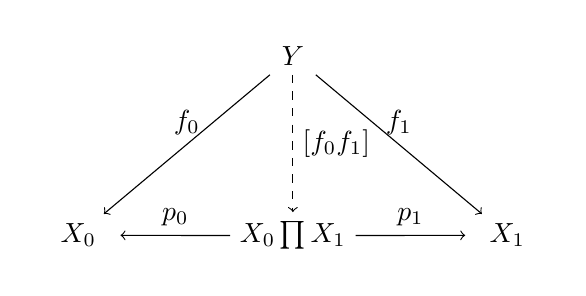
\begin{tikzpicture}
		\matrix (m) [matrix of math nodes, row sep=5em, column sep=4em, minimum width=3em]
		{
			& Y  & \\ 
			X_0  & X_0 \prod X_1 & X_1   \\
		};
		\path[->]
		(m-1-2) edge node [above] {$f_0$} (m-2-1)
		edge node [above] {$f_1$} (m-2-3)
		(m-2-2) edge node [above] {$p_0$} (m-2-1)
		edge node [above] {$p_1$} (m-2-3)
		;
		\path[dashed,->]
		(m-1-2) edge node [right] {$[f_0f_1]$} (m-2-2)
		;
		\end{tikzpicture} 
		\end{gathered}
		\]
In general
	\[
	\begin{gathered}
	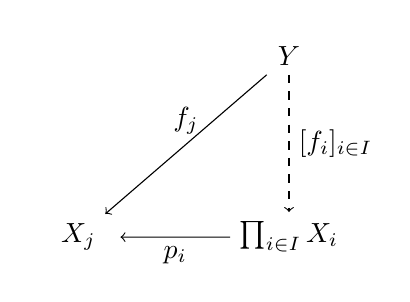
\begin{tikzpicture}
	\matrix (m) [matrix of math nodes, row sep=5em, column sep=4em, minimum width=3em]
	{
		& Y  \\ 
		X_j  & \prod_{i\in I} X_i   \\
	};
	\path[->]
	(m-1-2) edge node [above] {$f_j$} (m-2-1)
	(m-2-2) edge node [below] {$p_i$} (m-2-1)
	;
	\path[dashed,->]
	(m-1-2)        edge node [right] {$[f_i]_{i\in I}$} (m-2-2)
	;
	\end{tikzpicture}  
	\end{gathered}
	\]

\textbf{product} of $X_i$'s, 
\[ 
\prod_i X_i \equiv \prod_{i\in I} X_i
\]
given by 
\begin{equation}
\prod_i X_i := \lim_{ \longleftarrow } \alpha 
\end{equation}

When $X_i = X$, $\forall \, i \in I$, denote product by $X^{ \prod I} \equiv X^I$.  

	
\end{definition}

e.g. Cartesian product $P= A\times B$ of 2 sets $A,B$, $A,B \in \text{Obj}\textbf{Sets}$.  

Define 	
\[
\begin{gathered}
	\begin{aligned}
	& p:A\times B \to A \\
	& p(a,b) \mapsto a 
	\end{aligned} \qquad \, 
		\begin{aligned}
		& q:A\times B \to B \\
		& q(a,b) \mapsto b 
		\end{aligned}
\end{gathered}
\]
If $X \in \text{Obj}\textbf{Sets}$,  \\
if 
$	\begin{aligned} & \quad \\ 
& f: X \to A \\
& g : X  \to B 
\end{aligned}
$, then $\begin{aligned} & \quad \\ 
& \theta: X \to A\times B \\
& \theta : x \mapsto (f(x),g(x)) \in A\times B
\end{aligned}
$

\begin{proposition}[7.28 Rotman (2010); equivalence of products, if it exists]
If $A,B \in \text{Obj}\mathbf{C}$, then $\forall \, $ 2 products of $A$ and $B$, should they exist, are equivalent. 
\end{proposition}

\begin{proof}
	Suppose $C,D$ products of $A,B$.  Suppose products $\begin{aligned} & \quad \\ 
	& p_A : C \to A , \qquad \, & q_A: D\to A \\
	& p_B : C \to B , \qquad \, & q_B : D \to B \end{aligned}$  
	\[
	\begin{gathered}
	\begin{tikzpicture}
	\matrix (m) [matrix of math nodes, row sep=5em, column sep=4em, minimum width=3em]
	{
		& D  & \\ 
		A  & C & B   \\
	};
	\path[->]
	(m-1-2) edge node [above] {$q_A$} (m-2-1)
	edge node [above] {$q_B$} (m-2-3)
	(m-2-2) edge node [above] {$p_A$} (m-2-1)
	edge node [above] {$p_B$} (m-2-3)
	;
	\path[dashed,->]
	(m-1-2) edge node [right] {$\theta$} (m-2-2)
	;
	\end{tikzpicture} 
	\end{gathered}
	\]
	Just substitute $X=D$ in diagram above.  
	
	Then substitute again: 
	\[
	\begin{gathered}
	\begin{tikzpicture}
	\matrix (m) [matrix of math nodes, row sep=5em, column sep=4em, minimum width=3em]
	{
		& C  & \\ 
		A  & D & B   \\
	};
	\path[-{>[scale=3.0]}]
	(m-1-2) edge node [above] {$p_A$} (m-2-1)
	edge node [above] {$p_B$} (m-2-3) 
	(m-2-2) edge node [above] {$q_A$} (m-2-1)
	edge node [above] {$q_B$} (m-2-3)
	;
	\path[dashed,->]
	(m-1-2) edge node [right] {$\psi$} (m-2-2)
	;
	\end{tikzpicture} 
	\end{gathered}
	\]
	Then combine the 2 diagrams: $\psi \theta = 1_C$.  Likewise by label symmetry of $C,D$, $\theta \psi = 1_D$.  
	
	Then $C,D$ are equivalent.  

	
	\end{proof}

\subsubsection{Products of Modules and Sets}  

\begin{proposition}[7.29 Rotman (2010); products of R-modules are equivalent]
	If commutative ring $R$, \\
	R-modules $A,B$, \\
	then $\exists \, $ their (categorical) product $A\sqcup B$, in fact 
	\begin{equation}
	A \sqcap B \cong A\sqcup B
	\end{equation}
	
\end{proposition}

\begin{proof}
	If $A\sqcup B \cong M$, then 
	$\exists \, $ R-maps, $\begin{aligned} & \quad \\
		& i : S\to M \\ 
		& j : T \to M \end{aligned}$, \qquad \,  $\begin{aligned} & \quad \\
		& p : M\to S \\ 
		& q : M \to T \end{aligned}$
	s.t. $\begin{aligned} & \quad \\
	& pi = 1_A \\ 
	& qj = 1_B \end{aligned}$ \qquad \, and $\begin{aligned} & \quad \\
	& pj = 0 \\ 
	& qi = 0 \end{aligned}$, and $ip + jq = 1_M$, i.e.   
	
		\begin{tikzpicture}
		\matrix (m) [matrix of math nodes, row sep=5em, column sep=4em, minimum width=3em]
		{
			A & M & B \\ 
		};
		\path[->]
		($(m-1-2)+(0,-0.1)$) edge node [below] {$p$} ($(m-1-1.east)+(0,-0.1)$)
		edge node [below] {$q$} ($(m-1-3.west)+(0,-0.1)$) 
		($(m-1-1)+(0,0.1)$) edge node [above] {$i$} ($(m-1-2.west)+(0,0.1)$)
		($(m-1-3)+(0,0.1)$) edge node [above] {$j$} ($(m-1-2.east)+(0,0.1)$)
		;
		\end{tikzpicture} 
		
If module $X$, since $\begin{aligned}
& \quad \\ 
& f: X \to A \\
& g:X\to B
\end{aligned}	$ 
are homomorphisms, 

define 
$\begin{aligned}
& \theta: X \to A \sqcup B \\
& \theta(x) = if(x) + jg(x)
\end{aligned}
$
so that 
\[
	\begin{tikzpicture}
	\matrix (m) [matrix of math nodes, row sep=5em, column sep=4em, minimum width=3em]
	{
		& X  & \\ 
		A  & A\sqcup  & B   \\
	};
	\path[-{>[scale=4.0]}]
	(m-1-2) edge node [above] {$f$} (m-2-1)
	edge node [above] {$g$} (m-2-3) 
	(m-2-2) edge node [above] {$p$} (m-2-1)
	edge node [above] {$q$} (m-2-3)
	;
	\path[dashed,->]
	(m-1-2) edge node [right] {$\theta$} (m-2-2)
	;
	\end{tikzpicture} 
\]
since, $\forall \, x \in X$, 
\[
p\theta(x) = pif(x) + pjg(x) = pif(x) + 0 = f(x)
\]
since $ip + jq=1_{A\sqcup B}$  

\[
\psi = ip\psi + jq \psi = i f + jf = \theta
\]
so product is unique.  
	\end{proof}

\begin{definition}
	Let $R$ be commutative ring, \\
	let $\lbrace A_i : i \in I \rbrace$ be indexed family of $R$-modules.  
	
	\textbf{direct product} $\prod_{i\in I} A_i$ is cartesian product (i.e. set of all $I$-tuples $(a_i)$ whose $i$th coordinate $a_i$ lies in $A_i \quad \, \forall \, i$) with coordinate wise addition and scalar multiplication: 
	\[
	\begin{gathered}
	(a_i) + (b_i) = (a_i + b_i) \\
	r(a_i) = (ra_i)
	\end{gathered}
	\]
	where $r\in R$, $a_i, b_i \in A_i$, \, $\forall \, i $  
\end{definition}




cf. Thm. 7.32 of Rotman (2010) \cite{JRotman2010}
\begin{theorem}[7.32, Rotman]
	Let commutative ring $R$.  \\
	$\forall \, R$-module $A$, $\forall \,$ family $\lbrace B_i | i \in I \rbrace$ of $R$-modules,
	\begin{equation}
	\begin{gathered}
	\text{Hom}_R(A, \coprod_{i\in I} B_i ) \simeq \coprod_{i \in I} \text{Hom}_R(A,B_i)
	\end{gathered}
	\end{equation}
	via $R$-isomorphism
	\[
	\varphi : f\mapsto (p_if)
	\]
	where $p_i $ are projections of product $\coprod_{i\in I }B_i$
\end{theorem}

\begin{proof}
	Let $a\in A$, $f,g \in \text{Hom}_R(A,\coprod_{i\in I} B_i)$.
	\[
	\varphi(f+g)(a) = (p_i(f+g))(a) = (p_i(f(a) + g(a))) = (p_if + p_ig)(a)
	\]
	$\varphi$ additive.
	
	$\forall \, i, \, \forall \, r \in R$, $p_i rf = rp_i f$ (since product of $R$-modules, $\coprod_{i\in I}B_i$ is also an $R$-module of $\text{Obj}{}_R\textbf{Mod}$, by def. of product).
	\[
	\varphi rf \mapsto (p_i rf) = (r p_i f) = r(p_i f) = r\varphi(f)
	\]
	So $\varphi$ is $R$-map.
	
	If $(f_i) \in \coprod_i \text{Hom}{}_R(A,B_i)$, then $f_i : A\to B_i$ \, $\forall \, i$
	
	By Rotman's Prop. 7.31 (If family of $R$-modules $\lbrace A_i | i \in I \rbrace$, then direct product $C = \coprod_{i\in I} A_i$ is their product in ${}_R \textbf{Mod}$), \\
	\phantom{ \qquad \, } By def. or product, $\exists \, ! \, R$-map , \, $\theta : A \to \coprod_{i\in I} B_i$ s.t. $p_i \theta = f_i$ \, $\forall \, i$
	
	\[
	\begin{gathered}
	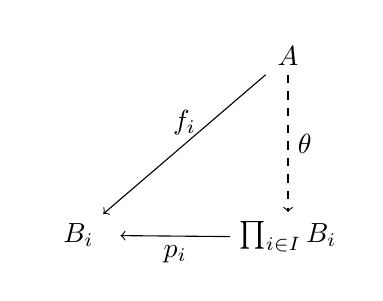
\begin{tikzpicture}
	\matrix (m) [matrix of math nodes, row sep=5em, column sep=4em, minimum width=3em]
	{
		& A  \\ 
		B_i  & \prod_{i\in I} B_i   \\
	};
	\path[->]
	(m-1-2) edge node [above] {$f_i$} (m-2-1)
	(m-2-2) edge node [below] {$p_i$} (m-2-1)
	;
	\path[dashed,->]
	(m-1-2)        edge node [right] {$\theta$} (m-2-2)
	;
	\end{tikzpicture}  
	\end{gathered}
	\]
	
	
	
	
	Then 
	\[
	f_i) = (p_i\theta) = \varphi(\theta)
	\]
	, and so $\varphi$ \emph{surjective}.
	
	Suppose $f\in \text{ker}\varphi$, so $\theta = \varphi(f) = (p_if)$.  Thus $p_i f=0$ \, $\forall \, i$
	
	\[
	\begin{gathered}
	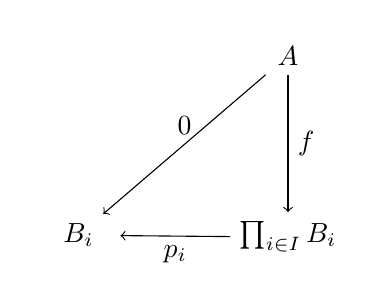
\begin{tikzpicture}
	\matrix (m) [matrix of math nodes, row sep=5em, column sep=4em, minimum width=3em]
	{
		& A  \\ 
		B_i  & \prod_{i\in I} B_i   \\
	};
	\path[->]
	(m-1-2) edge node [above] {$0$} (m-2-1)
	edge node [right] {$f$} (m-2-2)
	(m-2-2) edge node [below] {$p_i$} (m-2-1)
	;
	\end{tikzpicture}  
	\end{gathered}
	\]
	
	But $0$-homomorphism also makes this diagram commute, so uniqueness of homomorphism $A \to \prod B_i$ gives $f=0$.  
	
	
	
	
\end{proof}



%--------------------------------------------------------------------------------
% END of 20180202 
%-------------------------------------------------------------------------------





\part{Reading notes on Cox, Little, O'Shea's \emph{Ideals, Varieties, and Algorithms: An Introduction to Computational Algebraic Geometry and Commutative Algebra}}

\section{Geometry, Algebra, and Algorithms}

\subsection{Polynomials and Affine Space}

fields are important is that linear algebra works over \emph{any} field

\begin{definition}[2] set of all polynomials in $x_1 , \dots , x_n$ with coefficients in $k$, denoted $k[x_1, \dots , x_n]$

\end{definition}

polynomial $f$ \emph{divides} polynomial $g$ provided $g= fh$ for some $h \in k[x_1, \dots , x_n ]$

$k[x_1, \dots, x_n]$ satisfies all field axioms except for existence of multiplicative inverses; commutative ring, $k[x_1, \dots , x_n]$ \emph{polynomial ring}


\subsubsection*{Exercises for 1 }

\exercisehead{1}
$\mathbb{F}_2$ commutative ring since it's an abelian group under addition, commutative in multiplication, and multiplicative identity exists, namely $1$.  It is a field since for $1\neq 0$, the multiplicative identity is $1$.  

\exercisehead{2}
\begin{enumerate}
\item[(a)]
\item[(b)]
\item[(c)]
\end{enumerate}




\subsection{Affine Varieties }


\subsection{Parametrizations of Affine Varieties}


\subsection{Ideals}



\subsection{Polynomials of One Variable}




\section{Groebner Bases}

\subsection{Introduction}




\subsection{Orderings on the Monomials in $k[x_1, \dots , x_n]$ }




\subsection{A Division Algorithm in $k[x_1, \dots , x_n ]$ }



\subsection{Monomial Ideals and Dickson's Lemma }


\subsection{The Hilbert Basis Theorem and Groebner Bases}


\subsection{Properties of Groebner Bases}



\subsection{Buchberger's Algorithm}






\section{Elimination Theory}



\subsection{The Elimination and Extension Theorems}


\subsection{The Geometry of Elimination}



\section{The Algebra-Geometry Dictionary}


\subsection{Hilbert's Nullstellensatz}


\subsection{Radical Ideals and the Ideal-Variety Correspondence}



\section{Polynomial and Rational Functions on a Variety}


\subsection{Polynomial Mappings }


\section{Robotics and Automatic Geometric Theorem Proving}



\subsection{Geometric Description of Robots}






\part{Reading notes on Cox, Little, O'Shea's \emph{Using Algebraic Geometry}}

\textbf{Using Algebraic Geometry}.  David A. Cox.  John Little. Donal O'Shea. Second Edition.  Springer.  2005.  ISBN 0-387-20706-6 QA564.C6883 2004

\section{ Introduction }

\subsection{ Polynomials and Ideals }

\emph{monomial } 

\begin{equation}
  (1.1) \quad \quad \, x_1^{\alpha_1} \dots x_n^{\alpha_n}
\end{equation}

total degree of $x^{\alpha}$ is $\alpha_1 + \dots + \alpha_n \equiv |\alpha|$ \\



field $k$, $k[x_1 \dots x_n]$ collection of all polynomials in $x_1 \dots x_n$ with coefficients $k$.   \\

polynomials in $k[x_1 \dots x_n]$ can be added and multiplied as usual, so $k[x_1 \dots x_n]$ has structure of commutative ring (with identity) \\
however, only nonzero constant polynomials have multiplicative inverses in $k[x_1 \dots x_n]$, so $k[x_1 \dots x_n]$ not a field \\
\quad however set of rational functions $\lbrace f/g | f,g \in k[x_1 \dots x_n], \, g\neq 0\rbrace$ is a field, denoted $k(x_1 \dots x_n)$ \\

so
\[
f = \sum_{\alpha} c_{\alpha}x^{\alpha}
\]
where $c_{\alpha} \in k$

so

\[
f \in k [x_1 \dots x_n ] = \lbrace f | f = \sum_{\alpha} c_{\alpha} x^{\alpha} , x^{\alpha} = x_1^{\alpha_1} \dots x_n^{\alpha_n}, c_{\alpha} \in k \rbrace
\]

$f$ homogeneous if all monomials have same total degrees

polynomial $f$ is homogeneous if all monomials have the \emph{same total degree} \\

Given a collection of polynomials $f_1 \dots f_s \in k[x_1 \dots x_n]$, we can consider all polynomials which can be built up from these by multiplication by arbitrary polynomials and by taking sums

\begin{definition}[1.3] Let $f_1 \dots f_s \in k[x_1 \dots x_n]$ \\
Let $\langle f_1 \dots f_s \rangle = \lbrace p_1 f_1  + \dots + p_s f_s | p_i \in k[x_1 \dots x_n] \text{ for } i = 1 \dots s \rbrace$
\end{definition}


\exercisehead{1} 
\begin{enumerate}
\item[(a)] $x^2 = x \cdot ( x  -y^2 ) + y \cdot ( xy )$  
\item[(b)] 
\[
 p \cdot ( x - y^2 ) = p x - p y^2
\]
and for $p xy = (py)x$
\item[(c)] 
\[
p(y) ( x - y^2) = p(y)x - p(y) y^2 \notin \langle x^2, xy \rangle
\]
\end{enumerate}

\exercisehead{2} 
\[
\begin{gathered}
  \sum_{i=1}^s p_i f_i  + \sum_{j=1}^s q_j f_j = \sum_{i=1}^s (p_i + q_i )f_i, \quad \, p_i + q_i \in k[x_1 \dots x_n] \end{gathered}
\]
$\langle f_1 \dots f_s \rangle$ closed under sums in $k[x_1 \dots x_n]$ \\

If $f\in \langle f_1 \dots f_s \rangle$, \\
\phantom{If }$ p \in k [x_1 \dots x_n]$

\[
\begin{gathered}
p\cdot f = p \sum_{i=1}^s q_j f_j = \sum_{i=1}^s pq_j f_j, \quad \, pq_j \in k[x_1 \dots x_n] \text{ so }  \\
p\cdot f \in \langle f_1 \dots f_s \rangle
\end{gathered}
\]

Done.  \\

The 2 properties in Ex. 2 are defining properties of ideals in the ring $k[x_1 \dots x_n]$

\begin{definition}[1.5]
Let $I \subset k[x_1 \dots x_n]$, \, $I \neq \emptyset$ \\
$I$ ideal if 
\begin{enumerate}
\item[(a)] $f+ g \in I$, \, $\forall \, f,g \in I$ 
\item[(b)] $pf \in I$, \, $\forall \, f \in I$, arbitrary $p \in k[x_1 \dots x_n]$
\end{enumerate}
\end{definition}

Thus $\langle f_1 \dots f_s\rangle$ is an ideal by Ex. 2.  \\

we call it the ideal generated by $f_1 \dots f_s$.  

\exercisehead{3} Suppose $\exists \, $ ideal $J$, $f_1 \dots f_s \in J$ s.t. $J \subset \langle f_1 \dots f_s \rangle$ \\
if $f\in \langle f_1 \dots f_s \rangle$, $f = \sum_{i=1}^s p_i f_i$, \, $p_i \in k[x_1 \dots x_n]$ \\

$\forall \, i = 1 \dots s$, $p_i f_i \in J$ and so $\sum_{i=1}^s p_i f_i \in J$, by def. of $J$ as an ideal.

\[
\langle f_1 \dots f_s \rangle \subseteq J \quad \quad \, \Longrightarrow J = \langle f_1 \dots f_s \rangle
\]

$\Longrightarrow \langle f_1 \dots f_s \rangle$ is smallest ideal in $k[x_1 \dots x_n]$ containing $f_1 \dots f_s$


\exercisehead{4} For $\begin{aligned} & \quad \\
  & I = \langle f_1 \dots f_s \rangle \\
  & J = \langle g_1 \dots g_t \rangle \end{aligned}$ \\

 $I = J$ iff $s=t$ and $\forall \, f \in I$, $f = \sum_{i=1}^t q_i g_i$ and if $ 0  = \sum_{i=1}^t q_i g_i$, $q_i =0$, \, $\forall \, i = 1 \dots t$, and if $0 = \sum_{i=1}^s p_i f_i$, \, $p_i = 0$, \, $\forall \,  i = 1 \dots s$


\begin{definition}[1.6]
\[
\sqrt{I} = \lbrace g \in k[x_1\dots x_n] | g^m \in I \text{ for some } m \geq 1 \rbrace
\]
\end{definition}

e.g. $x+y \in \sqrt{ \langle x^2 + 3 xy , 3xy + y^2 \rangle }$

in $\mathbb{Q}[x,y]$ since 

\[
(x+y)^3 =x(x^2 + 3xy) + y(3xy + y^2) \in \langle x^2 + 3xy, 3xy + y^2\rangle
\]


%\begin{definition}[1.6]
%\[
%\sqrt{I } = \lbrace g \in k[x_1 \dots x_n ] | g^m \in I \text{ for some m } \geq 1 \rbrace
%\]
%\end{definition}

%e.g. $x+y \in \sqrt{ \langle x^2 + 3xy, 3xy + y^2 \rangle }$

%in $\mathbb{Q}[x,y]$ since

%\[
%(x+y)^3 = x(x^2 + 3xy) + y(3xy + y^2) \in \langle x^2 + 3xy, 3xy + y^2 \rangle
%\]

\begin{itemize}
\item (Radical Ideal Property) $\forall \, $ ideal $I\subset k[x_1 \dots x_n]$, $\sqrt{I}$ ideal, $\sqrt{I} \supset I$
\item \textbf{(Hilbert basis Thm.)} $\forall \, $ ideal $I\subset k[x_1\dots x_n]$ \\
$\exists \, $ finite generating set, \\
i.e. $\exists \, \lbrace f_1 \dots f_2 \rbrace \subset k [x_1 \dots x_n]$ s.t. $I=\langle f_1 \dots f_s \rangle$
\item (Division Algorithm in $k[x]$) $\forall \, f,g \in  k[x]$ (EY : in 1 variable) \\
$\forall \, f, g \in k[x]$ (in 1 variable )\\
$f= qg + r$, $\exists \, !$ quotient $q$, $\exists \, $ remainder $r$
\end{itemize}

\subsection{}

\subsection{Gr\"obner Bases}

\begin{definition}[3.1]
  Gr\"obner basis for $I$ $\equiv G = \lbrace g_1 \dots g_k \rbrace \subset I$ s.t. $\forall \, f \in I$, $\text{LT}(f)$ divisible by $\text{LT}(g_i)$ for some $i$
\end{definition}

\begin{itemize}
\item (Uniqueness of Remainders) let ideal $I\subset k[x_1 \dots x_n]$ \\
division of $f\in k[x_1 \dots x_n]$ by Gr\"o bner basis for $I$, produces $f=g+r$, $g\in I$, and no term in $r$ divisible by any element of $\text{LT}(I)$
\end{itemize}





\subsection{Affine Varieties}

affine $n$-dim. space over $k$ \quad \, $k^n = \lbrace (a_1 \dots a_n ) | a_1 \dots a_n \in k \rbrace$

$\forall \, $ polynomial $f\in k[x_1 \dots x_n ]$, $(a_1 \dots a_n) \in k^n$ \\
\phantom{ \quad } $f: k^n \to k$ \\
\phantom{ \quad } $f(a_1 \dots a_n)$ s.t. $x_i = a_i$ i.e. \\

if $f= \sum_{\alpha} c_{\alpha} x^{\alpha}$ for $c_{\alpha} \in k$, then  \\
\phantom{ \quad } $f(a_1 \dots a_n) =\sum_{\alpha} c_{\alpha}a^{\alpha} \in k$, where $a^{\alpha} = a_1^{\alpha_1} \dots a_n^{\alpha_n}$

\begin{definition}[4.1]
affine variety $\mathbf{V}(f_1 \dots f_s) = \lbrace ( a_1 \dots a_n) | (a_1 \dots a_n) \in k^n, \, f_1(x_1 \dots x_n) = \dots = f_s(x_1 \dots x_n) = 0 \rbrace$ \\
subset $V\subset k^n$ is affine variety if $V = V(f_1 \dots f_s)$ for some $\lbrace f_i \rbrace$, polynomial $f_i \in k[x_1 \dots x_n]$
\end{definition}

\begin{itemize}
  \item (Equal Ideals Have Equal Varieties) If $\langle f_1 \dots f_s \rangle = \langle g_1 \dots g_t \rangle$ in $k[x_1 \dots x_n]$, then $\mathbf{V}(f_1 \dots f_s) = \mathbf{V}(g_1 \dots g_t)$
\end{itemize}

so, recap \\
if $\langle f_1 \dots f_s \rangle = \langle g_1 \dots g_t \rangle $ in $k[x_1 \dots x_n]$, \\
then $V(f_1 \dots f_s) = V(g_1 \dots g_t)$   \\

Recall Hilbert basis Thm. $\forall \, $ ideal $I \subset k[x_1 \dots x_n]$ 
\[
I= \langle f_1 \dots f_s \rangle
\]
$\Longrightarrow $ if $I=J$, then $V(I) = V(J)$

think of $V$ defined by $I$, rather than $f_1 = \dots = f_s =0$

\exercisehead{3}

Recall Def. 1.5 Let $I\subset k[x_1 \dots x_n]$ \\
$I$ ideal if $\begin{aligned} & \quad \\
  & f + g \in I  \quad \, \forall \, f,g \in I \\
  & pf \in I, \quad \, \forall \, f \in I \text{ arbitrary } p \in k[x_1 \dots x_n]
\end{aligned}$

Let $f,g \in I(V)$ 
\[
\begin{gathered}
  (f+g)(a_1 \dots a_n) = f(a_1 \dots a_n) + g(a_1 \dots a_n) = 0 + 0 = 0 \quad \quad \, f+g \in I(V) \\ 
  pf(a_1 \dots a_n) = p(a_1 \dots a_n) f(a_1 \dots a_n) = 0 \quad \quad \, pf \in I(V)
\end{gathered}
\]
Then $I(V)$ an ideal.

%\exercisehead{3} Recall Def. 1.5. Let $I \subset k[x_1 \dots x_n]$, $I$ ideal if $\begin{aligned} & \quad \\
%  & f+g \in I \quad \, \forall \, f,g\in I \\
%  & pf \in I , \quad \, \forall \, f \in I, \text{ arbitrary } p \in k[x_1 \dots x_n ] \end{aligned}$

%Let $f,g \in I(V)$ 
%\[

$V = V(x^2)$ in $\mathbb{R}^2$ \\
$I=\langle x^2 \rangle$ in $\mathbb{R}[x,y]$, \, $I= \lbrace px^2 | p \in k[x,y]\rbrace$ \\
\phantom{ \quad } $I \subset I(V)$, since $px^2 = 0$ for $x^2=0$, $(0,b)$, \, $b\in \mathbb{R}$ \\
But $p(x,y) = x\in I(V)$, as 
\[
I(V) = \lbrace f \in k[x_1 \dots x_n] | f(a_1 \dots a_n)=0, \, \forall \, (a_1\dots a_n) \in V\rbrace
\]
\phantom{ \quad \quad } $p(0,b) = x = 0$

But $x\notin I$

\exercisehead{4} $I\subset \sqrt{I}$

Recall Def. 1.6 $\sqrt{I} = \lbrace g \in k[x_1 \dots x_n] |g^m \in I \text{ for some } m\geq 1\rbrace$ \\
$\forall \, f \in I$, $f=f^1$, $m=1$, so $f\in \sqrt{I}$, \quad \, $I\subset \sqrt{I}$ \\
\phantom{\quad \quad } Hilbert basis thm., $\forall \, $ ideal $I\subset k[x_1 \dots x_n]$ s.t. $I=\langle f_1 \dots f_s \rangle$ \\
\phantom{\quad } $V(I) = \lbrace (a_1 \dots a_n) |(a_1 \dots a_n) \in k^n, \, f_1(a_1\dots a_n) = \dots = f_s(a_1\dots a_n)=0\brace$ \\
$\mathbf{I}(\mathbf{V}(I)) = \lbrace f \in k[x_1 \dots x_n] | f(a_1 \dots a_n) =0 \quad \, \forall \, (a_1 \dots a_n) \in V(I) \rbrace$ \\
Let $g\in \sqrt{I}$, \, $g^m \in I$, \, $g^m=g^{m-1}g$  \\
\phantom{\quad \quad \,} $g^m(a_1 \dots a_n) =0 = g^{m-1}(a_1 \dots a_n)g(a_1 \dots a_n) =0$.  Then $g(a_1 \dots a_n)=0$ or $g^{m-1}(a_1\dots a_m)=0$ \\
\phantom{\quad }as $g^m\in I$, and $V(I)$ is s.t. $f_1(a_1 \dots a_n) = \dots = f_s(a_1 \dots a_n)=0$ for $I=\langle f_1 \dots f_s \rangle$

\begin{itemize}
  \item (Strong Nullstellensatz) if $k$ algebraically closed (e.g. $\mathbb{C}$), $I$ ideal in $k[x_1 \dots x_n]$, then 
\[
\mathbf{I}(\mathbf{V}(I) = \sqrt{I}
\]
\item (Ideal-variety correspondence) Let $k$ arbitrary field
\[
\begin{aligned}
  & I \subset I(V(I)) \\ 
  & V(I(V)) = V \quad \, \forall \, V
\end{aligned}
\]
\end{itemize}

\subsection*{Additional Exercises for Sec.4}

\exercisehead{6}



\section{ Solving Polynomial Equations}

\subsection{}

\subsection{Finite-Dimensional Algebras}

Gr\"obner basis $G = \lbrace g_1 \dots g_t \rbrace$ of ideal $I\subset k[x_1\dots x_n]$, \\
recall def.: Gr\"obner basis $G = \lbrace g_1 \dots g_t\rbrace \subset I$ of ideal $I$, \, $\forall \, f \in I$, $\text{LT}(f)$ divisible by $\text{LT}(g_i)$ for some $i$ \\
\phantom{\quad \, } $f \in k[x_1\dots x_n]$ divide by $G$ produces $f=g+r$, $g\in I$, $r$ not divisible by any $\text{LT}(I)$ uniqueness of $r$ \\
$f\in k[x_1 \dots x_n]$ divide by $G$, 

Recall from Ch. 1, divide $f\in k[x_1 \dots x_n]$ by $G$, the division algorithm yields

\begin{equation}
  (2.1)  \quad \quad \quad \, f = h_1 g_1 + \dots + h_t g_t + \overline{f}^G
\end{equation}
where remainder $\overline{f}^G$ is a linear combination of monomials $x^{\alpha} \notin \langle \text{LT}(I) \rangle $ \\
\phantom{\quad } since Gr\"obner basis, $f\in I$ iff $\overline{f}^G=0$

$\forall \, f \in k[x_1\dots x_n]$, we have coset $[f] = f+I = \lbrace f +h|h\in I\rbrace$ s.t. $[f]=[g]$ iff $f- g \in I$

We have a 1-to-1 correspondence 
\[
\begin{gathered}
\text{remainders } \leftrightarrow \text{ cosets } \\
\overline{f}^G \leftrightarrow [f]
\end{gathered}
\]
algebraic
\[
\begin{aligned}
  & \overline{f}^G + \overline{g}^G \leftrightarrow [f] + [g] \\ 
  & \overline{ \overline{f}^G \cdot \overline{g}^G } \leftrightarrow [f]\cdot [g]
\end{aligned}
\]
$B = \lbrace x^{\alpha} | x^{\alpha} \notin \langle \text{LT}(I) \rangle \rbrace$ is a basis of $A$, basis monomials, standard monomials

20141023 EY's take

$\forall \, [f] \in A = k[x_1 \dots x_n]/I$, \, $[f] = p_ib_i$; \, $b_i \in B = \lbrace x^{\alpha} | x^{\alpha} \notin \langle \text{LT}(I) \rangle \rbrace$ \\
For $I = \langle G \rangle$ \\
\phantom{\quad } e.g. $G=\lbrace x^2 + \frac{3}{2} xy + \frac{1}{2} y^2 - \frac{3}{2} x - \frac{3}{2} y, xy^2-x, y^3-y \rbrace$ \\
$\langle \text{LT}(I) \rangle = \langle x^2, xy^2,y^3 \rangle$ \\
e.g. $B=\lbrace 1,x,y,xy,y^2\rbrace$ \\
\phantom{\quad } $[f]\cdot[g] = [fg]$ \\
e.g. $f=x, \, g=xy, \, [fg] = [x^2y]$ \\
now $f=h_1g_1 + \dots +h_tg_t+ \overline{f}^G$

\subsection{}

\subsection{Solving Equations via Eigenvalues and Eigenvectors}


\section{ Resultants }

\section{Computation in Local Rings}

\subsection{Local Rings}


\begin{definition}[1.1]
  \[
k[x_1 \dots x_n]_{\langle x_1 \dots x_n \rangle} \equiv \lbrace \frac{f}{g} | \text{ rational functions } \frac{f}{g} \text{ of } x_1 \dots x_n \text{ with } g(p) \neq 0 \text{ at } p \rbrace
\]
\end{definition}

main properties of $k[x_1 \dots x_n]_{\langle x_1 \dots x_n \rangle }$

\begin{proposition}[1.2]
  Let $R= k[x_1 \dots x_n]_{\langle x_1 \dots x_n \rangle }$.  Then
\begin{enumerate}
\item[(a)] $R$ subring of field of rational functions $k(x_1 \dots x_n) \supset k[x_1 \dots x_n]$
\item[(b)] Let $M=\langle x_1 \dots x_n \rangle \subset R$ (ideal generated by $x_1 \dots X_n$ in $R$) \\
Then $\forall \, \frac{f}{g} \in R \backslash M$, $\frac{f}{g}$ unit in $R$ (i.e. multiplicative inverse in $R$)
\item[(c)] $M$ maximal ideal in $R$
\end{enumerate}
\end{proposition}


\exercisehead{1} if $p=(a_1 \dots a_n) \in k^n$, $R = \lbrace \frac{f}{g} | f,g\in k[x_1 \dots x_n] , \, g(p) \neq 0 \rbrace$ 
\begin{enumerate}
\item[(a)] $R$ subring of field of rational functions $k(x_1 \dots x_n)$ 
\item[(b)] Let $M$ ideal generated by $x_1 - a_1 \dots x_n -a_n$ in $R$  \\
Then $\forall \, \frac{f}{g} \in R\backslash M$, $\frac{f}{g}$ unit in $R$ (i.e. multiplicative inverse in $R$)
\item[(c)]  $M$ maximal ideal in $R$
\end{enumerate}


\begin{proof}
let $p = (a_1 \dots a_n) \in k^n$ \\
let $g_1(p) \neq 0$, $g_2(p) \neq 0$ 
\[
\begin{gathered}
  \frac{f_1}{g_1 } + \frac{f_2}{g_2} = \frac{f_1 g_2 + f_2 g_1}{ g_1 g_2 } \quad \quad \,  g_1(p)g_2(p) \neq 0 \text{ so } \frac{f_1}{g_1} + \frac{f_2}{g_2} \in R \\
 \frac{f_1}{g_1} \cdot \frac{f_2}{g_2} = \frac{f_1 f_2}{g_1 g_2} \quad \quad \, g_1(p) g_2(p) \neq 0 \text{ so } \frac{f_1}{g_1}\frac{f_2}{g_2} \in R
\end{gathered}
\]
$f= \frac{f}{I} \in R$, \quad \, $\forall \, f\in k[x_1 \dots x_n]$, so $k[x_1 \dots x_n]\subset R$

\end{proof}

EY : 20141027, to recap, 

Let $V = k^n$ \\
Let $p = (a_1 \dots a_n)$ \\
single pt. $\lbrace p \rbrace$ is (an example of) a variety \\
$I(\lbrace p \rbrace) = \lbrace x_1 -a_1 \dots x_n -a_n \rangle \subset k[x_1 \dots x_n]$ \\

$R \equiv k[x_1 \dots x_n]_{\langle x_1 - a_1 \dots x_n-a_n \rangle }$ 
\[
R = \lbrace \frac{f}{g} | \text{ rational function $\frac{f}{g}$ of $x_1 \dots x_n$, $g(p) \neq 0$, $p=(a_1 \dots a_n) $ } \rbrace
\]

Prop. 1.2. properties 

\begin{enumerate}
\item[(a)] $R$ subring of field of rational functions $k(x_1 \dots x_n)$ \quad \, $k(x_1 \dots x_n) \subset R$ 
\item[(b)] $M = \langle x_1 \dots a_1 \dots x_n -a_n \rangle \subset R$.  ideal generated by $x_1 - a_1 \dots x_n-a_n$ \\
Then $\forall \, \frac{f}{g} \in R\backslash M$, $\frac{f}{g}$ unit in $R$ ( $\exists \, $ multiplicative inverse in $R$ )
\item[(c)] $M$ maximal ideal in $R$. \\
in $R$ we allow denominators that are not elements of this ideal $I(\lbrace p \rbrace)$ 
\end{enumerate}

\begin{definition}[1.3] local ring is a ring that has exactly 1 maximal ideal \end{definition}

\begin{proposition}[1.4] ring $R$ with proper ideal $M\subset R$ is local ring if $\forall \, \frac{f}{g} \in R\backslash M$ is unit in $R$
\end{proposition}

localization Ex. 8, Ex. 9 \\
parametrization

\exercisehead{2} \[
\begin{aligned}
  & x = x(t) = \frac{-2t^2 }{1+t^2} \\ 
 &  y = y(t) = \frac{2t}{1+t^2}
\end{aligned}
\]
$k[t]_{\langle t \rangle}$ \quad \, $\frac{-2t^2}{1+t^2}$ rational function of $t$.  $1+t^2 \neq 0$

if $k = \mathbb{C}$ or $\mathbb{R}$ \\

Consider set of convergent power series in $n$ variables \\

\begin{equation}
(1.5) \quad \quad \,   k\lbrace x_1 \dots x_n \rbrace = \lbrace \sum_{\alpha \in \mathbb{Z}^n_{\geq 0}} c_{\alpha} x^{\alpha} | c_{\alpha} \in k, \text{ series converges in some open $U\ni 0 \in k^n $ } \rbrace
\end{equation}

Consider set $k[[x_1 \dots x_n]]$ of formal power series

\begin{equation}
  (1.6) \quad \quad \, k[[x_1 \dots x_n]] = \lbrace \sum_{\alpha \in \mathbb{Z}^n_{\geq 0}} c_{\alpha} x^{\alpha} | c_{\alpha} \in k \rbrace \text{ series need not converge }
\end{equation} 


variety $V$ \\

$k[x_1\dots x_n]/\mathbf{I}(V)$ \phantom{ \quad \quad \quad } variety $V$


\subsection{Multiplicities and Milnor Numbers}


if $I$ ideal in $k[x_1\dots x_n]$, then denote $Ik[x_1\dots x_n]_{\langle x_1 \dots x_n \rangle}$ ideal generated by $I$ in larger ring $k[x_1\dots x_n]_{\langle x_1 \dots x_n \rangle}$

\begin{definition}[2.1] Let $I$ $0$-dim. ideal in $k[x_1 \dots x_n]$, so $V(I)$ consists of finitely many pts. in $k^n$.  \\
Assume $(0 \dots 0) \in V(I)$ \\
multiplicity of $(0\dots 0)\in V(I)$ is 
\[
\text{dim}_k{ k[x_1\dots x_n]_{\langle x_1\dots x_n \rangle}} / Ik[x_!\dots x_n]_{\langle x_1 \dots x_n \rangle}
\]
\end{definition}


generally, if $p=(a_1 \dots a_n) \in V(I)$ \\
multiplicity of $p$, $m(p) = \text{dim}{ k[x_1 \dots x_n]_M } / Ik[x_1 \dots x_n]_M$

\[
\text{dim}{ k[x_1 \dots x_n]_M } / Ik[x_1 \dots x_n]_M
\]

localizing $k[x_1 \dots x_n]$ at maximal ideal $M = I(\lbrace p \rbrace) = \langle x_1 - a_1 \dots x_n-a_n \rangle$


\section{}

\section{}

\section{ Polytopes, Resultants, and Equations }

\section{ Polyhedral Regions and Polynomials }

\subsection{ Integer Programming }

Prop. 1.12. \\

Suppose 2 customers $A, B$ ship to same location \\
\quad A: ship 400 kg pallet taking up $2 \, m^3$ volume \\
\quad B: ship 500 kg pallet taking up $3 \, m^3$ volume \\

shipping firm trucks carry up to 3700 \, kg, up to $20 \, m^3$ \\

B's product more perishable, paying \$ 15 per pallet \\

A pays \$ 11 per pallet

How many pallets from A, B each in truck to maximize revenues?

\begin{equation}
(1.1) \quad \quad \, \begin{gathered}
    4A + 5B \leq 37 \\
    2A  + 3B \leq 20 \\
    A, B \in \mathbb{Z}^*_{ \geq 0 } \end{gathered}
\end{equation}

maximize $11 A + 15 B$ \\

integer programming. \\
max. or min. value of some linear function 

\[
l(A_1 \dots A_n) = \sum_{i=1}^n c_i A_i 
\]

on set $(A_1 \dots A_n) \in \mathbb{Z}^n_{ \geq 0}$ s.t. 


3. Finally, by introducing additional variables; rewrite linear constraint inequalities as equalities. The new variables are called ``slack variables''

\begin{equation}
(1.4) \quad \quad \, a_{ij} A_j = b_i, \quad \, A_j \in \mathbb{Z}_{\geq 0}
\end{equation}

introduce indeterminate $z_i$, \, $\forall \, $ equation in (1.4)

\[
z_i^{a_{ij} A_j} = z_i^{b_i}
\]

$m$ constraints

\[
\prod_{i=1}^m z_i^{a_{ij}A_j} = \prod_{i=1}^m z_i^{b_i} = \left( \prod_{i=1}^m z_i^{a_{ij}} \right)^{ A_j}
\]

\begin{proposition}[1.6]
  Let $k$ field, define $\varphi: k[w_1 \dots w_n] \to k[z_1 \dots z_m]$ by 
\[
\varphi(w_j) = \prod_{i=1}^m z_i^{a_{ij}} \quad \quad \quad \, \forall \, j = 1 \dots n 
\]

and 

\[
\varphi(g(w_1 \dots w_n) ) = g(\varphi(w_1) \dots \varphi(w_n))
\]
$\forall \, $ general polynomial $g\in k[w_1 \dots w_n]$

Then $(A_1 \dots A_n)$ integer pt. in feasible region iff $\varphi: w_1^{A_1} \dots w_n^{A_n} \mapsto z_1^{b_1} \dots z_m^{b_m}$



\end{proposition}

\exercisehead{3}

Now 

\[
\begin{gathered}
\varphi(w_j) = \prod_{i=1}^m z_i^{a_{ij}} \\
z_i^{a_{ij} A_j} = z_i^{b_i}
\end{gathered}
\]

If $(A_1 \dots A_n)$ an integer pt. in feasible region, $a_{ij} A_j = b_i$

\[
\begin{gathered}
z_i^{a_{ij}A_j } = z_i^{b_i} = \prod_{j=1}^n z_i^{a_{ij} A_j} \Longrightarrow \prod_{j=1}^n \prod_{i=1}^m (z_i^{a_{ij} })^{A_j} = \prod_{i=1}^m z_i^{b_i} = \prod_{j=1}^n \varphi(w_j)^{ A_j} = \prod_{j=1}^n \varphi(w_j)^{A_j} = \varphi\left( \prod_{j=1}^n w_j^{ A_j } \right) = \prod_{i=1}^m z_i^{b_i}
\end{gathered}
\]
since $\varphi(g(w_1 \dots w_n)) = g(\varphi(w_1) \dots \varphi(w_n))$ \\

If $\varphi: \prod_{j=1}^n w_j^{A_j} \mapsto \prod_{i=1}^m z_i^{b_i}$

\[
\varphi\left( \prod_{j=1}^n w_j^{A_j} \right) = \prod_{j=1}^n (\varphi(w_j))^{A_j} = \prod_{i=1}^m z_i^{b_i} = \prod_{j=1}^n \left( \prod_{i=1}^m z_i^{a_{ij}} \right)^{ A_j} \Longrightarrow \prod_{j=1}^n z_i^{a_{ij} A_j} = z_i^{b_i}
\]
or $a_{ij}A_j = b_i$.  So $(A_1\dots A_n)$ integer pt.  




\exercisehead{4} 
\[
\prod_{i=1}^m z_i^{b_i} = \prod_{i=1}^m \prod_{j=1}^n z_i^{ a_{ij} A_j } = \prod_{j=1}^n \left( \prod_{i=1}^m z_i^{a_{ij}} \right)^{A_j} = \prod_{j=1}^n \varphi(w_j)^{A_j} = \varphi\left( \prod_{j=1}^n w_j^{A_j} \right)
\]
So if given $(b_1 \dots b_m) \in \mathbb{Z}^m$, and for a given $a_{ij}$, $a_{ij}A_j = b_i$ \\

For $m\leq n$, then $a_{ij}$ is surjective, so $\exists \, A_j$ s.t. $\prod_{i=1}^m z_i^{b_i} = \varphi\left( \prod_{j=1}^n w_j^{A_j} \right)$



\begin{proposition}[1.8]
Suppose $f_1 \dots f_n \in k[z_1 \dots z_m]$ given \\
Fix monomial order in $k[z_1 \dots z_n, w_1 \dots w_n ]$ with elimination property: \\
$\forall \, $ monomial containing 1 of $z_i$ greater than any monomial containing only $w_j$ \\

Let $\mathcal{G}$ Gr\"{o}bner basis for ideal
\[
I = \langle f_1 - w_1 \dots f_n - w_n \rangle \subset k[z_1 \dots z_m, w_1 \dots w_n]
\]
$\forall \, f \in k[z_1 \dots z_m]$, let $\overline{f}^{ \mathcal{G}}$ be remainder on division of $f$ by $\mathcal{G}$ \\
Then
\begin{enumerate}
\item[(a)] polynomial $f$ s.t. $f\in k[f_1 \dots f_n]$ iff $g= \overline{f}^{ \mathcal{G}} \in k[w_1 \dots w_n]$
\item[(b)] if $\begin{aligned} & \quad \\
  & f \in k [f_1 \dots f_n ] \\
  & g = \overline{f}^{\mathcal{G}}\in k[ w_1 \dots w_n] \end{aligned}$ \quad as in part (a), \\

then $f = g(f_1 \dots f_n)$ , giving an expression for $f$ as polynomial in $f_j$
\item[(c)] if $\forall \, f_i, f$ monomials, $f\in k[f_1 \dots f_n]$, \\
then $g$ also a monomial.  
\end{enumerate}
\end{proposition}



\subsection{Integer Programming and Combinatorics}



\section{Algebraic Coding Theory}


\section{The Berlekamp-Massey-Sakata Decoding Algorithm}





\href{https://martinralbrecht.files.wordpress.com/2010/07/20131022_buchberger_dtu.pdf}{Gr\"{o}bner Bases, Martin R. Albrecht of the DTU Crypto Group}

\part{Conformal Field Theory : Virasoro Algebra}  

cf.  Schottenloher (2008)  \cite{Scho2008}




% 20170926  

\begin{definition}
	\textbf{extension} of $G$ by group $A$ is (given by) an \emph{exact sequence} of group homomorphisms.  
	\begin{tikzpicture}
	%\matrix(m)[matrix of math nodes, row sep=3em, column sep=3em, text height=1.5ex, text depth=0.25ex]
	\matrix(m)[matrix of math nodes, row sep=4em, column sep=4em]
	{
		1   &  A & E & G & 1 \\
	};
	%\path[->,font=\scriptsize]
	\path[->]
	(m-1-1) edge node[auto]{$$} (m-1-2)
	(m-1-2) edge node[auto]{$i$} (m-1-3)
	(m-1-3) edge node[auto]{$\pi$} (m-1-4)
	(m-1-4) edge node[auto]{$$} (m-1-5)	
	;
	\end{tikzpicture} 
\end{definition}
cf. Def. 3.1 of Schottenloher (2008)  \cite{Scho2008}.  

Recall that an exact sequence, if $\begin{aligned} & \quad \\
	& \text{im}(1\to A) = \text{ker}(i) \\
	& \text{im}(i) = \text{ker}(\pi) \\
	& \text{im}(\pi) = \text{ker}(G\to 1)
\end{aligned}$

By Thm., 
$1\to A \xrightarrow{i} E$ exact so $i$ injective.  \\
$E\xrightarrow{\pi} G \to 1$ exact so $\pi$ surjective.  

Extension is called \textbf{central} if $A$ abelian and image $\text{im}i$ is in center of $E$, i.e. 
$a\in A, b\in E \Longrightarrow i(a) b = bi(a)$.  

\subsubsection{Examples of extensions of $G$, and central extensions of $G$ (which has a particular $E$)}

e.g. central extension has form 
\[
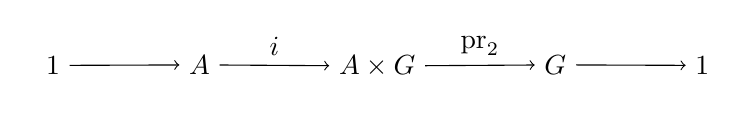
\begin{tikzpicture}
%\matrix(m)[matrix of math nodes, row sep=3em, column sep=3em, text height=1.5ex, text depth=0.25ex]
\matrix(m)[matrix of math nodes, row sep=4em, column sep=4em]
{
	1   &  A & A\times G & G & 1 \\
};
%\path[->,font=\scriptsize]
\path[->]
(m-1-1) edge node[auto]{$$} (m-1-2)
(m-1-2) edge node[auto]{$i$} (m-1-3)
(m-1-3) edge node[auto]{$\text{pr}_2$} (m-1-4)
(m-1-4) edge node[auto]{$$} (m-1-5)	
;
\end{tikzpicture} 
\]
where  \\
$\begin{aligned}
 i:A & \to A\times G \\
a & \mapsto (a,1) \end{aligned}$ 

\[
\begin{gathered}
i(a)(a',g) = (a,1)(a',g) = (aa',g) = \\
= (a'a,g\cdot 1) = (a',g)(a,1) = (a',g)i(a)
\end{gathered}
\]

Notice that what the \emph{exactness} property of an exact sequence does:
\[
\text{pr}_2i(a) = \text{pr}_2(a,1) = 1
\]

e.g. of a \text{nontrivial central extension} is exact sequence 
\begin{equation}
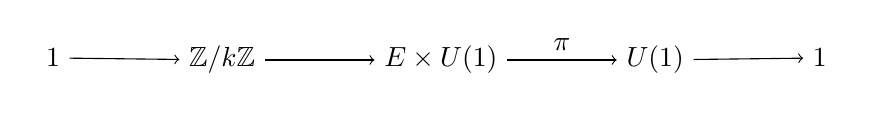
\begin{tikzpicture}
%\matrix(m)[matrix of math nodes, row sep=3em, column sep=3em, text height=1.5ex, text depth=0.25ex]
\matrix(m)[matrix of math nodes, row sep=4em, column sep=4em]
{
	1   &  \mathbb{Z}/k\mathbb{Z} & E\times U(1) & U(1) & 1 \\
};
%\path[->,font=\scriptsize]
\path[->]
(m-1-1) edge node[auto]{$$} (m-1-2)
(m-1-2) edge node[auto]{$$} (m-1-3)
(m-1-3) edge node[auto]{$\pi$} (m-1-4)
(m-1-4) edge node[auto]{$$} (m-1-5)	
;
\end{tikzpicture} 
\end{equation}
with $\pi(z) = z^k$ \, $\forall \, k \in \mathbb{N}$, $k\geq 2$, since $E=U(1)$ and $\mathbb{Z}/k\mathbb{Z}$ are not isomorphic.  

Also, homomorphism $\tau:U(1) \to E$ with $\pi \circ \tau = 1_{U(1)}$, doesn't exist, since there's no global $k$th root.  

EY : 20170926 It's that in integer division of the argument in a complex number $z\in U(1)$, and exponent multiplication by $k$, you go from 1 to many and many to 1, depending upon the "branch" you're mapping to for complex numbers.  

For $[n] \in \mathbb{Z}/k\mathbb{Z}$, 
\[
[n]\xmapsto[]{ i } \exp{ \left( \frac{ [n] }{ k} 2\pi i \right) }
\]
and so 
\[
\text{ker}\pi = \lbrace z | \pi(z) = 1 \rbrace \text{ so that } \text{ker}\pi = \lbrace z = \exp{ \left( \frac{i 2\pi n}{k} \right) } \rbrace
\]

e.g. \emph{Semidirect products}.  

group $G$ acting on another group $H$, by homomorphism   
\[
\tau : G \to \text{Aut}(H)
\]




%  20170926  of END 









\part{Algebraic Topology}  

cf. Bredon (1997) \cite{Bred1997}


\section{Simplicial Complexes}  

cf. pp. 245, from Sec. 21 Simplicial Complexes of Ch. 4 Homology Theory in Bredon (1997) \cite{Bred1997}

$\mathbf{v}_0, \dots \mathbf{v}_n \in \mathbb{R}^{\infty}$, "affinely independent" if they span an affine $n$-plane, i.e. 
\[
\text{ if } \left( \sum_{i=0}^n \lambda_i \mathbf{v}_i =0 , \, \sum_{i=0}^n \lambda_i = 0 \right), \text{ then } \Longrightarrow \forall \, \lambda_i = 0
\]
If not, then, e.g. $\lambda_0 \neq 0$, assume $\lambda_0 =-1$, and solve the equations to get 

\[
\begin{gathered}
\mathbf{v}_0 = \sum_{i=1}^n \lambda_i \mathbf{v}_i \\
\sum_{i=1}^n \lambda_i = 1
\end{gathered}
\]
i.e. $\mathbf{v}_0$ is in affine space spanned by $\mathbf{v}_1\dots \mathbf{v}_n$.  

If $\mathbf{v}_0, \dots \mathbf{v}_n$ affinely independent, then 
\begin{equation}
\sigma = ( \mathbf{v}_0, \dots \mathbf{v}_n) = \lbrace \sum_{i=0}^n \lambda_i \mathbf{v}_i | \sum_{i=0}^n \lambda_i = 1, \, \lambda_i \geq 0 \rbrace
\end{equation}
is "affine simplex" spanned by $\mathbf{v}_i$; also convex hull of $\mathbf{v}_i$.  

$\forall \, k \leq n$, $k$-face of $\sigma$ is any affine simplex of form $(\mathbf{v}_{i_1}, \dots \mathbf{v}_{i_k})$, where vertices all distinct, so are affinely independent.  

\begin{definition}
	(geometric) simplicial complex $K:= $ collection of affine simplices s.t. \begin{enumerate}
		\item $\sigma \in K \Longrightarrow $ any face of $\sigma \in K$; and 
		\item $\sigma, \tau \in K \Longrightarrow \sigma \bigcap \tau $ is a face of both $\sigma$ and $\tau$, or $\sigma \bigcap \tau =\emptyset$
	\end{enumerate}

If $K$ simplicial complex, $|K| = \bigcup \lbrace \sigma | \sigma \in K \rbrace \equiv $ "polyhedron" of $K$
\end{definition}

\begin{definition}[Def. 21.2 of Bredon (1997) \cite{Bred1997}]
	polyhedron $:= $ space $X$ if $\exists \, $ homeomorphism $h: |K| \xrightarrow{ \approx } X$ for some simplicial complex $K$.  
	$h,K$ is triangulation of $X$; (map $h$, complex $K$)
\end{definition}

Let $K$ finite simplicial complex.  \\
Choose ordering of vertices $\mathbf{v}_0,\mathbf{v}_1\dots $ of $K$.  \\
If $\sigma = (\mathbf{v}_{\sigma_0}, \dots \mathbf{v}_{\sigma_n})$ is simplex of $K$, where $\sigma_0 < \dots < \sigma_n$, then  \\
\phantom{If } let $f_{\sigma} : \Delta_n \to |K|$ be 
\[
f_{\sigma} = [\mathbf{v}_{\sigma_b}, \dots \mathbf{v}_{\sigma_n}]
\]
in notation of Def. 1.2.  Bredon (1997) \cite{Bred1997}.  

Then this gives CW-complex structure on $|K|$ with $f_{\sigma}$ as characteristic maps.  











\part{Graphs, Finite Graphs}

\section{Graphs, Finite Graphs, Trees }

Serre (1980) \cite{Serr1980}  

cf. Chapter I. Trees and Amalgams, Section 1 Amalgams, Subsection 1.1 Direct limits of Serre (1980) \cite{Serr1980}  


Let $(G_i)_{i\in I}$, family of groups.    

$\forall \, $ pair $(i,j)$, let $F_{ij} = $ set of homomorphisms of $G_i$ into $G_j$

Want: group $G= \varinjlim G_i$ and 
\[
\lbrace f_i | f_i : G_i \to G \rbrace \text{s.t. } f_j \circ f = f_i \quad \, \forall \, f \in F_{ij}
\]
group $G$ and family $\lbrace f_i\rbrace$ universal in that  

(*) if $H$ group, if $\lbrace h_i | h_i :G_i \to H ; h_j \circ f = h_i \qquad \, \forall \, f \in F_{ij} \rbrace$, \\
then $\exists \, ! h: G\to H$ s.t. $h_i = h\circ f_i$  \\
i.e. $\text{Hom}(G,H) \simeq \varprojlim \text{Hom}(G_i,H)$, the inverse limit being taken relative to $F_{ij}$.  \\
i.e. $G$ direct limit of $G_i$ relative to the $F_{ij}$.  

\begin{proposition}
	$\exists \, !$ pair $G$, family $(f_i)_{i\in I}$, i.e. (pair consisting of $G, (f_i)_{i\in I}$, unique up to unique isomorphism.  
\end{proposition}
\begin{proof}
Define $G$ by generators and relations.  \\
Take generating family to be disjoint union of those for $G_i$.  \\
relations - $xyz^{-1}$ where $x,y,z \in G_i$, $z=xy \in G_i$ \\
\phantom{relations - } $xy^{-1}$ where $x\in G_i$, $y \in G_j$, $y=f(x)$ for at least $f\in F_{ij}$.  

Thus, existence of $G,\lbrace f_i\rbrace$.  

$G$ represents functor $H\mapsto \varprojlim \text{Hom}{(G_i,H)}$.  

Thus, uniqueness (also from universal property).  
\end{proof}

e.g. groups $A,G_1,G_2$, homomorphisms $\begin{aligned} & \quad \\ 
& f_1 : A \to G_1 \\
& f_2 : A \to G_2 
\end{aligned}$.  

$G$ obtained by amalgamating $A$ in $G_1,G_2$ by $f_1,f_2 \equiv G_1 *_A G_2$.  \\
1 can have $G=\lbrace 1 \rbrace$, even though $f_1,f_2$ non-trivial.  

\emph{Application}: (Van Kampen Thm.)

Let topological space $X$ be covered by open $U_1,U_2$.   \\
Suppose $U_1,U_2, U_{12}=U_1\bigcap U_2$ arcwise connected.  

Let basept. $x\in U_{12}$.  

Then $\pi_1(X;x)$ obtained by taking 3 groups 
\[
\pi_1(U_1;x), \pi_1(U_2;x), \pi_1(U_{12};x)
\]
and amalagamating them according to homomorphism
\[
\begin{aligned}
& \pi_1(U_{12};x) \to \pi_1(U_1;x)  \\
& \pi_1(U_{12};x) \to \pi_1(U_2;x)
\end{aligned}
\]

\exercisehead{1}  
Let homomorphisms $\begin{aligned} & \quad \\
	& f_1 : A \to G_1 \\ 
	& f_2: A \to G_2 \end{aligned}
$
amalgam $G=G_1 *_A G_2$.  

Define subgroups $A^n,G_1^n, G_2^n$, of $A,G_1,G_2$ recursively by 
\[
\begin{aligned}
& A^1 = \lbrace 1 \rbrace \\
& G_1^1 = \lbrace 1 \rbrace \\ 
& G_2^1 = \lbrace 1 \rbrace \\ 
\end{aligned}
\]

$A^n = $ subgroup of $A$ generated by $f_1^{-1}(G_1^{n-1})$ and $f_2^{-1}(G_2^{n-1})$  
\[
G_1^n = \text{subgroup of $G_i$ generated by $f_i(A^n)$ }
\]

Let $A^{\infty}, G_i^{\infty}$ be unions of $A^n, G_i^n$ resp.  

Show that $f_i$ defines injection $A/A^{\infty} \to G_i/G_i^{\infty}$.  

So the amalgamation is $G \simeq G_1/G_1^{\infty} *_{A/A^{\infty}} G_2/G_2^{\infty}$.  

Take the first induction case (for intuition about the solution).  

\[
\begin{aligned}
	& A^2 = \langle f_1^{-1}( G_1^1), f_2^{-1}(G_2^1) \rangle = \langle f_1^{-1}(\lbrace 1 \rbrace), f_2^{-1}(\lbrace 1 \rbrace ) \rangle \\
	& G_i^2 = f_i(A^2)
\end{aligned}
\]
Let $f_i(a) = f_i(b) \in G_i/G_i^{\infty}$; $a,b\in A/A^{\infty}$.  

Then since $f_i(a),f_i(b) \in G_i/G_i^{\infty}$, $f_i(a),f_i(b) \in \lbrace gG_i^{\infty} | g\in G_i \rbrace$ (quotient is defined to be the set of all left cosets of $G_i^{\infty}$, which has to be a normal subgroup for $G_i/G_i^{\infty}$ to be a quotient group).  

Since $a,b \in A/A^{\infty}$, suppose we take $a,b\in A$.  

And suppose we take 
\[
\begin{aligned}
& 	f_i(a) = f_i(a)G_i^{\infty} = f_i(a) f_i(A^{n_a} ) = f_i(aA^{n_a}) \\ 
& 	f_i(b) = f_i(b)G_i^{\infty} = f_i(b) f_i(A^{n_b} ) = f_i(bA^{n_b})  
\end{aligned}
\]
Taking $f_i^{-1}$ (recall for group homomorphisms, they map inverse of element of 1st. group to inverse of image of this element).  

$aA^{n_a}=bA^{n_b}\in A/A^{\infty}$ (This is okay as we've "quotiented out $A^{\infty}$; so indeed, they're equal)


cf. Subsection 1.2 Structure of amalgams of Serre (1980) \cite{Serr1980} 

Suppose given group $A$, family of groups $(G_i)_{i\in I}$, and, $\forall \, i\in I$, injective homomorphism $A\to G_i$.  

$*_A G_i \equiv $ direct limit (cf. no. 1.1) of family $(A,G_i)$ with respect to these homomorphisms, call it \emph{sum} (in category theory sense, i.e. product) of $G_i$ with $A$ amalgamated.  

e.g. $A=\lbrace 1 \rbrace$, \\
$*G_i \equiv $ free product of $G_i$.  

\subsubsection{reduced word}  

$\forall \, i \in I$, choose set $S_i$ of right coset representations of $G_i$ modulo $A$, 

assume $1 \in S_i$, 

$(a,s)\mapsto as$ is bijection of $A\times S_i$ onto $G_i$,  \\
$A\times (S_i-\lbrace 1 \rbrace) \to G_i-A$ (onto)

Let $\mathbf{i} = (i_1\dots i_n)$, $n\geq 0$, $i_j \in I$, s.t. 
\begin{equation}
i_m \neq i_{m+1} \text{ for } 1 \leq m \leq n-1
\end{equation}
cf. (T) of Serre (1980) \cite{Serr1980}.  

So \emph{reduced word} $m$ is defined as 
\[
m = (a;s_1\dots s_n)
\]
where $a\in A, s_1\in S_{i_1} \dots s_n \in S_{i_n}$, and $s-j \neq 1\, \forall \, j$.  

$f\equiv $ canonical homomorphism of $A$ into group $G= *_A G_i$ \\ 
$f_i \equiv $ canonical homomorphism of $G_i$ into group $G= *_A G_i$

EY : 20170611 (Further explanations, basic examples, from me):  

Given $A, \lbrace G_i\rbrace_{i\in I}$, injective (group) homomorphisms $\lbrace f_i: A \to G_i\rbrace_i$.  

$G_i \backslash f_i(A) = \lbrace f_i(A)g | g\in G_i\rbrace$.  

Right coset representation of $f_i(A)g\mapsto g$.  

e.g. $A,G_1,G_2$, $\begin{aligned} & \quad \\
	& f_1:A \to G_1 \\
		& f_2 : A\to G_2 \end{aligned}$.  
		
	\[
	\begin{aligned}
	& G_1\backslash f_1(A) = \lbrace f_1(A)g| g\in G_1\rbrace \\
	& G_2\backslash f_2(A) = \lbrace f_2(A)g | g\in G_2 \rbrace
	\end{aligned}
	\]

$\mathbf{i} = (i_1\dots i_n)$, $i_j\in I$, $i_m\neq i_{m+1}$ for $1\leq m \leq n-1$.  

Consider $(1212\dots 12)$  

$m=(a;f_1 g_2 f_3 g_4 \dots f_{2n-1}, g_{2n})$ where $f$'s $\in S_1 \subset G_1$, $g$'s $\in S_2 \subset G_2$.  

and so 
\begin{definition}[reduced word]
	\textbf{reduced word} of type $\mathbf{i}$, $m$, \begin{equation}
	m=(a;s_1\dots s_n)
	\end{equation}
	where $a\in A, s_1 \in S_{i_1}, \dots s_n \in S_{i_n}$, $s_j\neq 1$ \, $\forall \, j$, \\
	\phantom{where } $\mathbf{i} = (i_1\dots i_n)$, $i_j \in I$, s.t. $i_m \neq i_{m+1}$ for $1\leq m \leq n-1$, \\
	with $S_i = \lbrace g | g\in f_i(A)g \in f_i(A) G_i\rbrace$  
\end{definition}




\begin{theorem}[1 of Serre (1980) \cite{Serr1980} ]
	$\forall \, g \in G$, $\exists \, $ sequence $\mathbf{i}$ s.t. $i_m \neq i_{m+1}$ for $1\leq m \leq n-1$ and 
	
	reduced word 
	\[
	m = (a;s_1\dots s_n) 
	\]
	of type $\mathbf{i}$ s.t. 
	\[
	g = f(a)f_{i_1}(s_1) \dots f_{i_n}(s_n)
	\]
\end{theorem}

Furthermore, $\mathbf{i}$ and $m$ unique.  

\emph{Remark}.  Thm. 1 implies $f;f_i$ injective.  

Then identify $A$ and $G_i$ with images $f(A), f_i(G_i)$ in $G$, and reduced decomposition (*) of $g\in G$ 
\[
g = as_1\dots s_n, \quad \, a\in A, \, s_1 \in S_{i_1} - \lbrace 1 \rbrace \dots s_n \in S_{i_n} - \lbrace 1 \rbrace
\]
Likewise, $G_i \bigcap G_j = A$ if $i\neq j$.  

In particular, $S_i - \lbrace 1 \rbrace$ pairwise disjoint in $G$.  

\begin{proof}
Let $X_i \equiv $set of reduced words of type $\mathbf{i}$, $X = \coprod X_i$.  

Make $G$ act on $X$.  

In view of universal property of $G$, sufficient to make $\forall \, i, G_i$ act, 

check action induced on $A$ doesn't depend on $i$  

Suppose then that $i\in I$, and let $Y_i = $ set of reduced words of form $(1;s_1 \dots s_n)$, with $i_1\neq i$.  

EY : 20170611

Recall that 
\[
S_i = \lbrace g| g\in f_i(A) g \in f_i(A) G_i \rbrace
\]
\[
\begin{aligned}
	& A \times S_i \to G_i \text{ onto } \\ 
	& A\times (S_i - \lbrace 1 \rbrace) \to G_i - A \text{ onto } \\ 
	& (a,s) \mapsto as \text{ bijection }
\end{aligned}
\]

Let $Y_i = $ set of reduced words of form $(1; s_1 \dots s_n) = \lbrace (1;s_1 \dots s_n) | 1\in A; s_1 \in S_{i_1}\dots s_n \in S_{i_n} ; \mathbf{i} = (i_1\dots i_n), \, i_j \in I \text{ s.t. } i_m \neq i_{m+1} \text{ for } 1\leq m \leq n -1 \rbrace$.  

\[
\begin{gathered}
\begin{gathered}
A \times Y_i \to X = \coprod_i X_i \\
(a,(1; s_1 \dots s_n)) \mapsto (a; s_1 \dots s_n)
\end{gathered} \\
\begin{gathered}
A\times \lbrace S_i - \lbrace 1 \rbrace ) \times Y_i \to X \\
((a,s), (1;s_1 \dots s_n)) \mapsto (a;s,s_1\dots s_n)
\end{gathered}
\end{gathered}
\]
and remember that $X_i = $ set of reduced words of type $\mathbf{i}$.  

It's clear that this yields a bijection $A\times Y_i \bigcup A\times (S_i - \lbrace 1 \rbrace) \times Y_i \to X$.  

Let $x\in X$.  Then $x\in X_{\mathbf{i}}$ for some $\mathbf{i}$.  So $x$ is a reduced word of type $\mathbf{i}$: $x = (a;s_1\dots s_n)$.  Then clearly $x = (a;s_1\dots s_n) \mapsto (a,(1;s_1\dots s_n)) \in A\times Y_i$.  







\end{proof}


cf. pp. 13, Sec. 2. Trees, 2.1 Graphs of Serre (1980) \cite{Serr1980}

\begin{definition}[1. of Serre (1980) \cite{Serr1980}]
	\textbf{graph} $\Gamma = (X,Y, Y\to X\times X, Y\to Y)$, where $\begin{aligned} & \quad \\
		& \text{ set } X = \text{ vert } \Gamma \\ 
		& \text{ set } Y = \text{ edge } \Gamma \end{aligned}$  

\[
\begin{aligned}
& Y \to X\times X \\ 
& y\mapsto (o(y), t(y)) \\
& Y\to Y \\
& y\mapsto \overline{y}
\end{aligned}
\]
s.t. $\forall \, y \in Y$, $\overline{ \overline{y}} = y$, $\overline{y} \neq y$, $o(y) = t(\overline{y})$.  

vertex $P \in X$ of $\Gamma$. 

(oriented) edge $y\in Y$, $\overline{y} \equiv $ inverse edge.  

origin of $y := $ vertex $o(y) = t(\overline{y})$.  

terminus of $y:= $ vertex $t(y) = o(\overline{y})$   

extremities of $y:= \lbrace o(y),t(y)\rbrace$  

If 2 vertices \textbf{adjacent}, they're extremities of some edge.  

orientation of graph $\Gamma = Y_+ \subset Y = \text{ edge } \Gamma$ s.t. $Y = Y_+ \coprod \overline{Y}_+$.  It always exists.  

oriented graph defined, up to isomorphism, by giving 2 sets $X,Y_+$ and $Y+ \to X\times X$.  
	
	corresponding set of edges is $Y = Y_+\coprod \overline{Y}_+$ where $\overline{Y}_+ \equiv $ copy of $Y_+$  
\end{definition}

\subsubsection{Realization of a Graph}

cf. Realization of a Graph in Serre (1980) \cite{Serr1980}.  

Let graph $\Gamma$, $X = \text{vert}\Gamma$, $Y = \text{edge}\Gamma$.

topological space $T = X \coprod Y \times [0,1]$, where $X,Y$ provided with discrete topology.  

Let $R$ be finest equivalence relation on $T$ for which 
\begin{equation}
\begin{gathered} \begin{aligned}
	& (y,t) \equiv (\overline{y}, 1-t) \\ 
	& (y,0) \equiv o(y) \\
	& (y,1) \equiv t(y)
\end{aligned} \qquad \, \forall \, y \in Y, \, \forall \, t \in [0,1]
\end{gathered}
\end{equation}

quotient space $\text{real}(\Gamma) = T/R $ is \emph{realization} of graph $\Gamma$.  (realization is a functor which commutes with direct limits).  

Let $n\in \mathbb{Z}^+$.  Consider oriented graph of $n+1$ vertices $0,1,\dots n$,  \\

\begin{definition}
	path (of length $n$) in graph $\Gamma$ is morphism $c$ of $\mathbf{\text{Path}}_n$ into $\Gamma$  
\end{definition}

orientation given by $n$ edges $[i,i+1]$, $0\leq i <n$, $\begin{aligned} & \quad \\
& o([i,i+1]) = i \\
& t([i,i+1]) = i+1 \end{aligned}$  

For $n\geq 1$, \\
$(y_1\dots y_n)$ sequence of edges $y_i = c([i-1,i])$ s.t. 
\[
t(y_i) = o(y_{i+1}), \qquad \, 1 \leq i < n \text{ determine } c
\]
If $P_i = c(i)$,  \\
$c$ is a path from $P_0$ to $P_n$, and $P_0$ and $P_n$ are \emph{extremities of the path $c$}.  

pair of form $(y_i,y_{i+1})=(y_i, \overline{y}_i)$ in path is \textbf{backtracking}.  

path (of length $n-2$), from $P_0$ to $P_n$ given (for $n>2$) by $(y_1\dots y_{i-1}, y_{i+2}\dots y_n)$  

If $\exists \, $ path from $P$ to $Q$ in $\Gamma$, $\exists \, $ one without backtracking (by induction)  

direct limit $\mathbf{\text{Path}}_{\infty} = \varinjlim \mathbf{\text{Path}}_n$ provides notion of infinite path.  \\
$\mathbf{\text{Path}}_{\infty} \ni $ infinite sequence $(y_1,y_2 , \dots)$ of edges s.t. $t(y_i) = o(y_{i+1})$ \, $\forall \, i \geq 1$.  


\begin{definition}[connected graph; Def. 3 of Serre (1980) \cite{Serr1980}]
	graph connected if $\forall \, $ 2 vertices, 2 vertices are extremities of at least 1 path.  
	
	maximal connected subgraphs (under relation of inclusion) are \emph{connected components} of graph.  
\end{definition}

\subsubsection{Circuits}  

Let $n\in \mathbb{Z}^+$, $n\geq 1$.  

Consider \\
set of vertices $\mathbb{Z}/n\mathbb{Z}$, orientation given by $n$ edges $[i,i+1]$, $(i\in \mathbb{Z}/n\mathbb{Z})$ with $\begin{aligned} & \quad \\
 & o([i,i+1]) = i \\
 & t([i,i+1]) = i+1 \end{aligned}$

\begin{definition}[circuit; Def. 4 of Serre (1980) \cite{Serr1980}]
	circuit (length $n$) in graph is subgraph isormorphic to $\mathbf{\text{Circ}}_n$.  
\end{definition}
i.e. subgraph = path $(y_1\dots y_n)$, without backtracking, s.t. $P_i = t(y_i)$, \, $(1\leq i \leq n)$ distinct, s.t. $P_n = o(y_1)$

$n=1$ case: $\mathbf{\text{Circ}}_1$, $\mathbb{Z}/\mathbb{Z} = \lbrace 0 \rbrace$, $1$ edge, $[0,1]$, $0 \in \mathbb{Z}/1\mathbb{Z}$, $\begin{aligned} & \quad \\
	& o([0,1]) = 0 \\
	& t([0,1]) = 1 \end{aligned}$  
	
	Note $\mathbf{\text{Circ}}_1$ has automorphism of order 2, which changes its orientation, i.e. \\
	$\exists \, $ automorphism $\sigma \in \text{Aut}( \mathbf{\text{Circ}}_1) $ s.t. $|\sigma | = 2$, i.e. $\sigma^2=1$.  \\
	loop $:= $ circuit of length $1$; so loop $\in \overline{ \mathbf{\text{Circ}} }_1$.  
	
	path $(y_1)$, $P_1 = t(y_1) = o(y_1)$.  
	
	$n=2$ case: $\mathbf{\text{Circ}}_2$, $\mathbb{Z}/2\mathbb{Z} = \lbrace 0 ,1\rbrace$, 2 edges $[0,1], [1,2]$,  \\
	path $(y_1,y_2)$, $(1\leq i \leq 2)$, $\begin{aligned} & \quad \\
		& P_1 = t(y_1) \\
		& P_2 = t(y_2) = o(y_1) \end{aligned}$  
		
		
	

\subsection{Combinatorial graphs}

Let $(X,S)\equiv $ simplicial complex of dim. $\leq 1$, with \\
$X \equiv $ set \\
$S \equiv $ set of subsets of $X$ with $1$ or $2$ elements, containing all the 1-element subsets.  

associates with it a graph $\Gamma = (X, \lbrace (P,Q) \rbrace)$.  

$X$ is its set of vertices.  

edges $=\lbrace (P,Q)\in X\times X\rbrace$ s.t. $P\neq Q$, $\lbrace P ,Q \rbrace \in S$, with $\overline{(P,Q)} = (Q,P)$
\[
\begin{aligned}
& o(P,Q) = P \\
& t(P,Q) = Q
\end{aligned}
\]

In this graph, 2 edges with same origin and same terminus are equal.  This is equivalent to (see following Def.)

\begin{definition}[combinatorial; Def. 5 of Serre (1980) \cite{Serr1980}]
	graph is combinatorial if it has no circuit of length $\leq 2$
\end{definition}
Conversely, it's easy to see that 

every combinatorial graph $\Gamma$ derived (up to isomorphism) by construction above from simplicial complex $(X,S)$, where \\
$X = \text{vert} \Gamma$ \\
$S=$ set of subset $\lbrace P,Q \rbrace$ of $X$ s.t. $P$ and $Q$ either adjacent or equal.  



\end{multicols*}

\begin{thebibliography}{9}


\bibitem{JRotman2010}
Joseph J. Rotman, \textbf{Advanced Modern Algebra} (Graduate Studies in Mathematics) 2nd Edition, American Mathematical Society; 2 edition (August 10, 2010), ISBN-13: 978-0821847411



%--------------------------------------------------------------------------------
% 20180203 
%-------------------------------------------------------------------------------


\bibitem{KaSch2006}
Masaki Kashiwara and Pierre Schapira. \textbf{Categories and Sheaves}.  \emph{Grundlehren der mathematischen Wissenschaften}.  Volume 332.  2006. Springer-Verlag Berlin Heidelberg.  eBook ISBN 978-3-540-27950-1
        


%--------------------------------------------------------------------------------
% END of 20180203 
%-------------------------------------------------------------------------------



\bibitem{CLS2005}
David A. Cox.  John Little. Donal O'Shea. \textbf{Using Algebraic Geometry}.  Second Edition.  Springer.  2005.  ISBN 0-387-20706-6 QA564.C6883 2004

\bibitem{CLS2015}
David Cox, John Little, Donal O'Shea. \textbf{Ideals, Varieties, and Algorithms: An Introduction to Computational Algebraic Geometry and Commutative Algebra}, Fourth Edition, Springer

\bibitem{Bred1997}
Glen E. Bredon.  \textbf{Topology and Geometry}. Graduate Texts in Mathematics (Book 139).  Springer; Corrected edition (October 17, 1997).  ISBN-13: 978-0387979267


\bibitem{Serr1980}  
Jean-Pierre Serre (Author), J. Stilwell (Translator).  \textbf{Trees} (Springer Monographs in Mathematics) 1st ed. 1980. Corr. 2nd printing 2002 Edition.  ISBN-13: 978-3540442370





\end{thebibliography}


\end{document}
